
\documentclass[
10pt, % Main document font size
a4paper, % Paper type, use 'letterpaper' for US Letter paper
oneside, % One page layout (no page indentation)
]{scrartcl}

\usepackage{amsmath} 
\usepackage{adjustbox}
\usepackage{textcomp}
\usepackage{environ}
\usepackage{tikz}
\usepackage{graphics}
\usepackage{pgfplots} 
\pgfplotsset{compat=1.9}

\title{Draft for master thesis} % The article title

\author{Henrique Rocha} 
\date{} 
\begin{document}

	\maketitle % Print the title/author/date block

	%----------------------------------------------------------------------------------------
	%	INTRODUCTION
	%----------------------------------------------------------------------------------------

	\section{Test}

\subsection{Usability Test}

	\subsubsection{Task 1 (Video)}
		Register User, add the coordinator as a friend, create a room, add the coordinator to the room wait for the coordinator to join the room and change for the individual view.
		
	\subsubsection{Task 2 (Tags)}
		The coordinator creates previously a room with existing content, namely, tags and subtitles.
		The user task is to enter in the public room and search by "Cauchy Rule" get an url for that time and send it back to the other users.
		Next the user should create a tag on exact arrival time (when he entered the room).
		
		
	\subsubsection{Task 3 (Content)}
		The user must create a subtitle with 10s duration at the time of arrival with the content "I've just arrived" and search for the previously created tag

	\subsubsection{Task 4 (Colaborative)}

			
\subsection{Performance Test}

	\begin{center}
	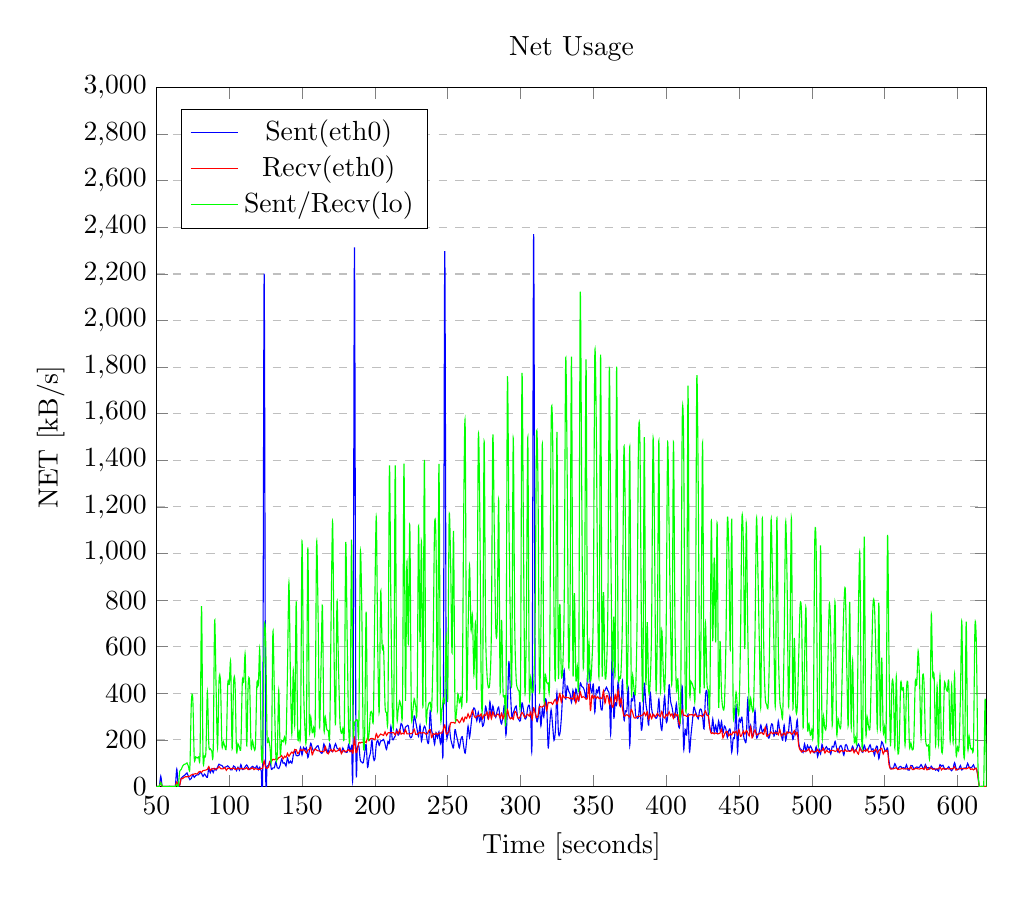
\begin{tikzpicture}
	\begin{axis}[
	    width=\textwidth,
	    title={Net Usage},
	    xlabel={Time [seconds]},
	    ylabel={NET [kB/s]},
	    xmin=50, xmax=620,
	    ymin=0, ymax=3000,
	    xtick={0,50,...,10000},
	    ytick={0,200,...,10000},
	    legend pos=north west,
	    ymajorgrids=true,
	    grid style=dashed,
	] 
		\addplot[smooth,color=blue]
		coordinates {
(0,0.0)(1,3.221)(2,4.828)(3,0.932)(4,0.0)(5,0.324)(6,0.112)(7,0.0)(8,0.0)(9,0.0)(10,0.07)(11,0.0)(12,0.29)(13,2.82)(14,0.0)(15,0.0)(16,0.0)(17,0.0)(18,0.0)(19,0.0)(20,0.0)(21,0.0)(22,0.0)(23,1.111)(24,0.0)(25,0.0)(26,0.0)(27,0.0)(28,0.0)(29,0.0)(30,0.0)(31,0.0)(32,0.0)(33,0.0)(34,0.0)(35,0.0)(36,0.0)(37,11.96)(38,0.0)(39,0.14)(40,2.961)(41,2.936)(42,0.042)(43,0.0)(44,0.0)(45,0.29)(46,26.679)(47,0.0)(48,0.0)(49,0.0)(50,0.0)(51,0.0)(52,0.0)(53,44.075)(54,0.0)(55,0.0)(56,0.0)(57,0.0)(58,0.0)(59,0.0)(60,0.0)(61,0.0)(62,0.0)(63,0.0)(64,75.087)(65,2.669)(66,6.674)(67,35.28)(68,42.19)(69,46.482)(70,51.428)(71,58.404)(72,43.034)(73,29.396)(74,34.766)(75,50.881)(76,39.184)(77,47.065)(78,50.037)(79,50.429)(80,60.565)(81,56.319)(82,43.366)(83,53.46)(84,45.177)(85,39.713)(86,78.982)(87,59.194)(88,74.369)(89,59.743)(90,76.717)(91,70.045)(92,82.674)(93,95.825)(94,91.975)(95,90.206)(96,80.923)(97,82.226)(98,85.358)(99,88.646)(100,82.36)(101,71.409)(102,71.835)(103,88.115)(104,83.636)(105,68.115)(106,82.829)(107,69.924)(108,94.129)(109,72.48)(110,76.182)(111,85.087)(112,92.608)(113,82.472)(114,73.334)(115,81.311)(116,86.608)(117,81.037)(118,78.416)(119,88.795)(120,71.844)(121,82.867)(122,66.636)(123,80.155)(124,2200.895)(125,109.158)(126,87.665)(127,90.552)(128,109.081)(129,73.408)(130,79.743)(131,80.434)(132,105.789)(133,80.632)(134,76.978)(135,92.063)(136,117.941)(137,99.992)(138,102.069)(139,87.757)(140,122.434)(141,99.883)(142,108.701)(143,99.671)(144,134.413)(145,156.268)(146,133.033)(147,131.622)(148,134.924)(149,167.659)(150,135.098)(151,167.993)(152,156.675)(153,167.04)(154,124.265)(155,151.186)(156,185.55)(157,165.204)(158,151.511)(159,161.658)(160,170.257)(161,175.317)(162,153.563)(163,144.809)(164,145.252)(165,182.696)(166,155.167)(167,159.82)(168,142.854)(169,182.743)(170,156.316)(171,149.313)(172,166.093)(173,183.593)(174,164.468)(175,160.401)(176,154.93)(177,147.259)(178,165.352)(179,149.071)(180,148.275)(181,147.36)(182,179.644)(183,151.387)(184,173.332)(185,148.067)(186,2314.092)(187,176.147)(188,169.546)(189,174.15)(190,113.153)(191,104.865)(192,102.143)(193,143.056)(194,180.792)(195,82.718)(196,121.826)(197,145.043)(198,199.072)(199,121.984)(200,116.578)(201,183.013)(202,197.619)(203,176.783)(204,196.059)(205,196.604)(206,202.064)(207,182.014)(208,159.007)(209,194.41)(210,185.777)(211,258.745)(212,201.453)(213,206.014)(214,216.817)(215,245.681)(216,220.243)(217,232.81)(218,270.153)(219,258.805)(220,233.199)(221,254.718)(222,259.946)(223,260.368)(224,215.145)(225,209.961)(226,231.039)(227,303.209)(228,278.526)(229,244.869)(230,214.692)(231,263.758)(232,194.644)(233,235.737)(234,258.825)(235,243.547)(236,195.449)(237,192.414)(238,325.215)(239,238.825)(240,222.835)(241,181.095)(242,231.339)(243,208.769)(244,235.462)(245,185.057)(246,226.99)(247,257.107)(248,2297.494)(249,387.533)(250,225.043)(251,259.742)(252,207.237)(253,180.866)(254,168.157)(255,243.589)(256,219.641)(257,192.775)(258,165.781)(259,201.766)(260,213.87)(261,170.387)(262,143.226)(263,196.361)(264,259.204)(265,210.645)(266,262.014)(267,315.296)(268,337.434)(269,325.708)(270,281.851)(271,318.31)(272,278.204)(273,302.132)(274,259.123)(275,276.54)(276,344.022)(277,313.532)(278,290.025)(279,364.724)(280,305.17)(281,345.598)(282,314.956)(283,296.487)(284,324.869)(285,340.558)(286,291.778)(287,268.339)(288,307.782)(289,347.509)(290,220.484)(291,334.267)(292,535.603)(293,417.112)(294,301.308)(295,315.922)(296,333.443)(297,345.54)(298,298.659)(299,285.836)(300,284.44)(301,358.781)(302,331.012)(303,291.041)(304,296.834)(305,338.915)(306,348.917)(307,300.937)(308,271.191)(309,2371.073)(310,505.384)(311,291.655)(312,291.431)(313,346.168)(314,259.771)(315,336.32)(316,298.394)(317,376.71)(318,346.39)(319,166.329)(320,259.296)(321,329.368)(322,265.747)(323,198.129)(324,245.662)(325,401.934)(326,235.358)(327,225.436)(328,290.792)(329,404.288)(330,499.987)(331,375.674)(332,431.843)(333,411.02)(334,398.018)(335,360.807)(336,412.8)(337,372.513)(338,419.079)(339,389.728)(340,367.314)(341,442.447)(342,429.814)(343,424.961)(344,408.892)(345,376.516)(346,476.207)(347,505.019)(348,428.673)(349,402.466)(350,439.326)(351,318.396)(352,411.128)(353,402.213)(354,427.9)(355,345.482)(356,328.328)(357,403.025)(358,411.811)(359,425.906)(360,410.928)(361,388.306)(362,228.563)(363,642.046)(364,302.657)(365,360.576)(366,350.616)(367,448.868)(368,374.814)(369,344.927)(370,454.037)(371,286.032)(372,324.898)(373,326.944)(374,423.724)(375,176.252)(376,364.806)(377,368.206)(378,405.86)(379,308.924)(380,294.388)(381,297.768)(382,360.524)(383,242.232)(384,296.124)(385,443.448)(386,359.088)(387,317.92)(388,263.59)(389,404.004)(390,334.908)(391,303.994)(392,305.72)(393,292.544)(394,303.868)(395,375.788)(396,283.252)(397,241.476)(398,317.942)(399,387.728)(400,280.039)(401,300.338)(402,436.11)(403,366.66)(404,340.92)(405,305.08)(406,296.324)(407,356.212)(408,285.328)(409,251.162)(410,308.775)(411,429.534)(412,161.565)(413,245.454)(414,221.168)(415,310.835)(416,150.272)(417,217.54)(418,279.313)(419,340.175)(420,323.647)(421,307.571)(422,290.743)(423,327.049)(424,331.394)(425,301.083)(426,247.86)(427,390.308)(428,406.591)(429,302.021)(430,252.736)(431,234.209)(432,289.662)(433,233.485)(434,262.172)(435,230.601)(436,281.281)(437,242.814)(438,279.169)(439,230.087)(440,259.794)(441,246.571)(442,210.146)(443,240.225)(444,241.511)(445,147.507)(446,206.635)(447,213.714)(448,344.593)(449,146.341)(450,283.618)(451,276.913)(452,297.384)(453,223.61)(454,196.97)(455,200.456)(456,371.711)(457,240.872)(458,262.857)(459,225.55)(460,222.989)(461,326.203)(462,214.096)(463,218.91)(464,236.62)(465,264.225)(466,232.467)(467,245.137)(468,238.926)(469,266.597)(470,210.915)(471,214.243)(472,260.764)(473,266.858)(474,216.624)(475,238.007)(476,223.637)(477,281.689)(478,235.185)(479,224.442)(480,198.544)(481,264.178)(482,196.9)(483,229.215)(484,235.593)(485,300.137)(486,255.501)(487,201.942)(488,227.218)(489,236.936)(490,286.242)(491,188.418)(492,161.625)(493,157.397)(494,145.962)(495,183.259)(496,151.919)(497,176.416)(498,161.431)(499,173.655)(500,162.434)(501,149.246)(502,143.933)(503,170.444)(504,127.802)(505,160.167)(506,139.165)(507,180.778)(508,156.057)(509,160.638)(510,170.941)(511,159.238)(512,162.207)(513,138.985)(514,172.634)(515,169.66)(516,193.647)(517,166.349)(518,147.295)(519,167.808)(520,176.175)(521,159.941)(522,133.922)(523,177.008)(524,176.558)(525,155.167)(526,153.525)(527,153.891)(528,172.842)(529,153.327)(530,152.668)(531,166.963)(532,182.193)(533,168.304)(534,155.097)(535,146.379)(536,177.355)(537,156.777)(538,153.925)(539,163.97)(540,178.914)(541,157.066)(542,161.759)(543,133.102)(544,166.292)(545,171.761)(546,119.539)(547,155.469)(548,192.349)(549,178.854)(550,158.685)(551,151.9)(552,165.115)(553,109.427)(554,75.92)(555,79.328)(556,77.956)(557,98.149)(558,83.73)(559,74.629)(560,83.435)(561,86.312)(562,79.603)(563,80.696)(564,76.478)(565,93.495)(566,70.563)(567,70.917)(568,90.363)(569,89.285)(570,76.055)(571,79.718)(572,84.087)(573,81.59)(574,83.242)(575,94.168)(576,82.711)(577,75.476)(578,94.211)(579,78.555)(580,81.397)(581,74.916)(582,87.194)(583,77.93)(584,77.678)(585,70.183)(586,74.854)(587,66.069)(588,93.905)(589,87.037)(590,91.372)(591,77.397)(592,73.554)(593,77.153)(594,85.383)(595,74.217)(596,67.971)(597,76.209)(598,102.255)(599,79.044)(600,71.35)(601,75.786)(602,90.259)(603,70.983)(604,78.48)(605,79.474)(606,80.553)(607,99.295)(608,82.941)(609,81.606)(610,83.039)(611,93.261)(612,75.315)(613,78.642)(614,43.984)(615,0.0)(616,0.0)(617,0.0)(618,0.0)(619,0.0)(620,0.0)(621,0.0)(622,0.0)(623,0.0)(624,0.0)(625,0.0)(626,0.0)(627,0.0)(628,0.0)(629,0.0)(630,0.0)(631,0.0)(632,0.0)(633,0.0)(634,0.0)(635,0.0)(636,0.0)(637,0.0)(638,0.0)(639,0.214)(640,3.581)(641,2.308)(642,0.0)(643,0.0)(644,0.042)(645,0.0)(646,0.0)(647,0.0)(648,0.0)(649,0.0)(650,0.0)(651,0.0)(652,0.0)(653,0.0)(654,0.0)(655,0.0)
		};	
		\addlegendentry{Sent(eth0)}

		\addplot[smooth,color=red]
		coordinates {
(0,0.0)(1,2.524)(2,4.734)(3,20.472)(4,0.042)(5,0.486)(6,0.154)(7,0.042)(8,0.042)(9,0.042)(10,0.112)(11,0.042)(12,0.619)(13,7.583)(14,0.042)(15,0.042)(16,0.042)(17,0.042)(18,0.042)(19,0.042)(20,0.042)(21,0.042)(22,0.0)(23,2.887)(24,0.0)(25,0.0)(26,0.0)(27,0.0)(28,0.0)(29,0.0)(30,0.0)(31,0.0)(32,0.0)(33,0.0)(34,0.0)(35,0.0)(36,0.0)(37,4.577)(38,0.0)(39,0.135)(40,2.137)(41,2.538)(42,0.042)(43,0.0)(44,0.0)(45,0.0)(46,19.885)(47,0.0)(48,0.0)(49,0.0)(50,0.0)(51,0.0)(52,0.0)(53,17.321)(54,0.0)(55,0.0)(56,0.0)(57,0.0)(58,0.0)(59,0.0)(60,0.0)(61,0.0)(62,0.0)(63,0.649)(64,19.214)(65,7.052)(66,5.624)(67,34.381)(68,33.657)(69,38.749)(70,42.237)(71,41.726)(72,42.887)(73,44.551)(74,50.095)(75,51.07)(76,53.977)(77,55.062)(78,53.432)(79,62.129)(80,64.978)(81,60.653)(82,68.215)(83,69.131)(84,71.048)(85,73.397)(86,85.508)(87,69.099)(88,75.032)(89,77.629)(90,73.865)(91,76.116)(92,76.832)(93,85.936)(94,76.986)(95,75.61)(96,76.521)(97,81.853)(98,69.552)(99,78.651)(100,77.167)(101,77.266)(102,76.049)(103,79.236)(104,73.518)(105,74.154)(106,79.712)(107,75.074)(108,75.765)(109,77.776)(110,74.252)(111,76.324)(112,81.219)(113,72.707)(114,76.292)(115,76.287)(116,80.468)(117,72.288)(118,77.382)(119,74.852)(120,73.649)(121,74.216)(122,76.721)(123,79.462)(124,110.18)(125,80.734)(126,78.151)(127,82.894)(128,108.062)(129,107.7)(130,117.111)(131,114.798)(132,118.96)(133,115.712)(134,123.454)(135,127.101)(136,132.84)(137,118.993)(138,129.877)(139,124.951)(140,142.408)(141,129.584)(142,140.706)(143,148.064)(144,142.232)(145,158.758)(146,158.076)(147,141.509)(148,148.086)(149,158.899)(150,153.911)(151,159.101)(152,153.802)(153,143.575)(154,156.053)(155,159.224)(156,169.207)(157,136.301)(158,154.021)(159,160.612)(160,156.105)(161,153.047)(162,152.616)(163,150.092)(164,150.98)(165,149.01)(166,171.591)(167,145.296)(168,140.097)(169,151.241)(170,158.772)(171,149.821)(172,159.625)(173,149.816)(174,152.183)(175,155.295)(176,165.311)(177,140.999)(178,153.243)(179,154.699)(180,148.724)(181,153.43)(182,158.345)(183,150.209)(184,155.903)(185,144.855)(186,210.544)(187,145.863)(188,157.849)(189,188.588)(190,186.442)(191,189.869)(192,188.381)(193,193.215)(194,188.196)(195,210.29)(196,197.047)(197,205.385)(198,206.476)(199,204.476)(200,200.123)(201,227.06)(202,209.719)(203,217.889)(204,225.483)(205,221.959)(206,219.785)(207,234.488)(208,219.451)(209,230.515)(210,230.805)(211,230.388)(212,231.078)(213,230.916)(214,221.592)(215,236.317)(216,226.581)(217,242.884)(218,224.614)(219,228.681)(220,225.378)(221,244.015)(222,226.287)(223,225.966)(224,226.137)(225,227.45)(226,230.623)(227,245.313)(228,224.338)(229,223.753)(230,229.464)(231,232.459)(232,228.987)(233,231.424)(234,230.426)(235,224.865)(236,226.643)(237,238.542)(238,244.132)(239,210.222)(240,227.014)(241,223.999)(242,228.841)(243,223.062)(244,229.353)(245,229.748)(246,228.899)(247,243.869)(248,264.092)(249,225.844)(250,229.55)(251,238.552)(252,272.501)(253,274.11)(254,275.031)(255,271.532)(256,287.762)(257,282.723)(258,273.67)(259,282.716)(260,295.54)(261,278.257)(262,298.376)(263,292.124)(264,312.025)(265,295.173)(266,306.827)(267,326.724)(268,305.864)(269,295.088)(270,300.806)(271,306.174)(272,301.171)(273,312.326)(274,291.43)(275,307.569)(276,305.341)(277,319.657)(278,291.347)(279,321.826)(280,290.965)(281,319.678)(282,302.808)(283,301.905)(284,310.393)(285,310.086)(286,293.668)(287,314.743)(288,290.986)(289,311.421)(290,292.982)(291,329.66)(292,303.859)(293,290.273)(294,296.849)(295,288.358)(296,320.317)(297,317.306)(298,295.224)(299,292.518)(300,303.679)(301,317.97)(302,308.714)(303,296.939)(304,306.018)(305,310.192)(306,302.315)(307,319.857)(308,288.642)(309,337.618)(310,316.07)(311,297.4)(312,303.647)(313,342.886)(314,340.922)(315,342.113)(316,345.839)(317,360.185)(318,326.688)(319,360.51)(320,359.32)(321,361.232)(322,353.011)(323,365.59)(324,373.726)(325,353.661)(326,374.239)(327,399.04)(328,362.408)(329,392.488)(330,380.255)(331,383.88)(332,381.68)(333,381.146)(334,376.841)(335,379.662)(336,373.669)(337,400.044)(338,358.481)(339,388.16)(340,370.216)(341,406.197)(342,382.106)(343,386.025)(344,382.268)(345,375.968)(346,380.049)(347,439.852)(348,326.637)(349,390.863)(350,378.741)(351,389.722)(352,378.529)(353,385.778)(354,376.913)(355,380.628)(356,377.012)(357,411.155)(358,357.415)(359,389.223)(360,385.964)(361,354.632)(362,381.989)(363,340.478)(364,350.833)(365,394.106)(366,366.412)(367,412.475)(368,349.395)(369,378.871)(370,333.501)(371,302.714)(372,304.888)(373,308.553)(374,304.215)(375,297.949)(376,331.093)(377,316.294)(378,294.938)(379,293.513)(380,300.578)(381,301.793)(382,301.73)(383,305.107)(384,307.415)(385,317.403)(386,303.927)(387,320.583)(388,289.352)(389,310.406)(390,291.273)(391,310.717)(392,299.074)(393,302.63)(394,313.525)(395,303.501)(396,300.781)(397,322.062)(398,299.047)(399,294.037)(400,309.831)(401,303.179)(402,320.683)(403,303.734)(404,311.658)(405,292.436)(406,313.936)(407,303.7)(408,309.018)(409,267.01)(410,301.569)(411,328.915)(412,304.892)(413,306.012)(414,301.369)(415,300.93)(416,308.467)(417,307.596)(418,309.358)(419,302.383)(420,311.655)(421,300.707)(422,301.122)(423,304.157)(424,304.254)(425,299.553)(426,311.187)(427,324.214)(428,305.918)(429,302.921)(430,249.828)(431,227.495)(432,231.082)(433,225.779)(434,230.093)(435,227.331)(436,226.192)(437,229.487)(438,246.628)(439,208.927)(440,224.359)(441,234.688)(442,235.988)(443,217.764)(444,226.661)(445,221.438)(446,234.92)(447,229.429)(448,236.633)(449,221.746)(450,244.195)(451,215.589)(452,222.258)(453,238.115)(454,224.876)(455,240.251)(456,231.703)(457,217.276)(458,255.479)(459,208.702)(460,228.63)(461,242.718)(462,221.415)(463,225.94)(464,226.37)(465,231.74)(466,229.452)(467,223.731)(468,254.019)(469,216.605)(470,219.778)(471,223.953)(472,233.926)(473,226.464)(474,230.884)(475,228.716)(476,232.66)(477,221.788)(478,244.58)(479,216.929)(480,224.154)(481,230.096)(482,219.874)(483,234.649)(484,229.705)(485,233.718)(486,224.349)(487,227.03)(488,239.36)(489,221.74)(490,232.376)(491,175.101)(492,156.406)(493,148.304)(494,154.986)(495,150.417)(496,152.161)(497,154.46)(498,161.714)(499,144.217)(500,154.97)(501,147.058)(502,149.551)(503,149.799)(504,159.146)(505,146.673)(506,152.196)(507,154.099)(508,164.76)(509,143.486)(510,156.023)(511,149.082)(512,146.859)(513,155.283)(514,155.158)(515,154.161)(516,150.386)(517,153.247)(518,162.544)(519,145.743)(520,154.68)(521,152.248)(522,150.598)(523,157.378)(524,150.964)(525,152.578)(526,151.001)(527,152.896)(528,161.806)(529,144.9)(530,157.164)(531,149.024)(532,138.844)(533,164.782)(534,152.769)(535,149.619)(536,156.122)(537,151.174)(538,161.459)(539,147.473)(540,150.085)(541,152.708)(542,149.265)(543,153.854)(544,159.768)(545,143.73)(546,154.643)(547,159.581)(548,164.152)(549,139.51)(550,153.723)(551,150.775)(552,154.039)(553,94.079)(554,75.846)(555,75.176)(556,75.924)(557,78.5)(558,80.687)(559,73.008)(560,74.226)(561,74.853)(562,77.798)(563,75.301)(564,75.68)(565,75.173)(566,77.548)(567,74.313)(568,84.935)(569,72.585)(570,72.83)(571,77.63)(572,76.984)(573,75.851)(574,74.89)(575,77.728)(576,77.312)(577,73.101)(578,85.885)(579,71.475)(580,73.232)(581,80.89)(582,78.377)(583,73.729)(584,74.647)(585,75.56)(586,75.572)(587,76.15)(588,84.529)(589,71.147)(590,78.316)(591,73.999)(592,76.043)(593,77.271)(594,74.889)(595,76.048)(596,75.984)(597,76.545)(598,84.749)(599,70.301)(600,73.752)(601,75.924)(602,75.946)(603,77.443)(604,75.847)(605,77.218)(606,75.674)(607,78.329)(608,83.189)(609,73.331)(610,75.837)(611,71.482)(612,76.477)(613,76.915)(614,45.909)(615,0.0)(616,0.0)(617,0.0)(618,0.0)(619,0.0)(620,0.0)(621,0.0)(622,0.0)(623,0.0)(624,0.0)(625,0.0)(626,0.0)(627,0.0)(628,0.0)(629,0.0)(630,0.0)(631,0.0)(632,0.0)(633,0.0)(634,0.0)(635,0.0)(636,0.0)(637,0.0)(638,0.0)(639,0.371)(640,2.019)(641,2.486)(642,0.0)(643,0.0)(644,0.042)(645,0.0)(646,0.0)(647,0.0)(648,0.0)(649,0.0)(650,0.0)(651,0.0)(652,0.0)(653,0.0)(654,0.0)(655,0.0)
		};
		\addlegendentry{Recv(eth0)}

		\addplot[smooth,color=green]
		coordinates {
(0,0.0)(1,0.0)(2,0.0)(3,0.0)(4,0.0)(5,0.1)(6,9.4)(7,9.9)(8,9.9)(9,9.9)(10,9.9)(11,9.9)(12,9.8)(13,9.9)(14,4.245)(15,0.0)(16,0.0)(17,0.0)(18,0.0)(19,1.445)(20,0.0)(21,0.0)(22,0.0)(23,0.0)(24,1.445)(25,0.0)(26,0.0)(27,0.0)(28,0.0)(29,1.445)(30,0.0)(31,0.0)(32,0.0)(33,0.0)(34,1.445)(35,0.0)(36,0.0)(37,0.0)(38,0.0)(39,1.445)(40,0.0)(41,0.0)(42,0.0)(43,0.0)(44,7.862)(45,22.594)(46,0.0)(47,0.0)(48,0.0)(49,1.445)(50,0.156)(51,0.0)(52,0.0)(53,16.473)(54,1.853)(55,0.0)(56,0.0)(57,0.0)(58,0.0)(59,1.445)(60,0.0)(61,0.0)(62,0.0)(63,1.3)(64,8.508)(65,0.0)(66,64.134)(67,72.558)(68,87.254)(69,94.843)(70,96.499)(71,101.373)(72,86.569)(73,82.492)(74,360.157)(75,376.309)(76,122.513)(77,127.188)(78,122.304)(79,127.172)(80,150.222)(81,774.438)(82,132.746)(83,130.66)(84,150.2)(85,406.02)(86,179.145)(87,162.203)(88,152.438)(89,152.696)(90,712.809)(91,422.567)(92,167.071)(93,452.171)(94,449.211)(95,180.143)(96,191.766)(97,171.598)(98,174.595)(99,439.309)(100,438.428)(101,531.576)(102,161.097)(103,443.446)(104,441.167)(105,156.45)(106,183.94)(107,168.84)(108,172.484)(109,448.965)(110,447.951)(111,563.666)(112,175.601)(113,433.946)(114,446.651)(115,171.94)(116,196.85)(117,164.83)(118,177.021)(119,438.98)(120,435.006)(121,584.769)(122,164.451)(123,143.225)(124,662.871)(125,636.347)(126,214.548)(127,204.843)(128,169.993)(129,125.056)(130,664.57)(131,399.83)(132,133.872)(133,141.285)(134,414.771)(135,142.058)(136,198.513)(137,192.057)(138,213.039)(139,200.172)(140,495.102)(141,875.419)(142,483.317)(143,224.478)(144,499.265)(145,264.197)(146,794.199)(147,230.413)(148,235.954)(149,248.413)(150,1053.859)(151,458.656)(152,249.053)(153,234.695)(154,1026.492)(155,265.89)(156,299.022)(157,230.802)(158,254.225)(159,269.86)(160,1043.095)(161,744.001)(162,253.949)(163,503.663)(164,776.132)(165,256.088)(166,296.89)(167,245.183)(168,239.252)(169,225.349)(170,746.791)(171,1138.939)(172,568.198)(173,267.814)(174,795.773)(175,526.644)(176,279.076)(177,228.676)(178,249.598)(179,244.156)(180,1044.014)(181,632.395)(182,251.276)(183,247.982)(184,1060.077)(185,255.206)(186,275.15)(187,283.901)(188,285.475)(189,246.823)(190,995.61)(191,770.487)(192,207.854)(193,219.999)(194,750.168)(195,235.29)(196,227.069)(197,318.172)(198,314.287)(199,297.679)(200,799.997)(201,1155.507)(202,585.269)(203,319.875)(204,837.587)(205,600.806)(206,590.866)(207,346.14)(208,318.41)(209,328.061)(210,1373.172)(211,784.77)(212,330.555)(213,327.881)(214,1378.624)(215,354.966)(216,327.466)(217,367.457)(218,342.231)(219,353.523)(220,1385.493)(221,370.987)(222,964.239)(223,612.129)(224,1122.298)(225,332.934)(226,322.598)(227,376.879)(228,346.787)(229,348.074)(230,1118.087)(231,621.226)(232,1051.884)(233,340.953)(234,1401.93)(235,347.946)(236,330.049)(237,355.038)(238,361.782)(239,334.759)(240,599.96)(241,1119.333)(242,1034.665)(243,324.549)(244,1384.576)(245,349.636)(246,327.494)(247,378.171)(248,373.349)(249,645.384)(250,372.915)(251,1152.981)(252,968.219)(253,574.112)(254,1093.935)(255,338.736)(256,315.574)(257,397.77)(258,359.89)(259,382.015)(260,394.034)(261,1177.688)(262,1553.69)(263,387.95)(264,672.978)(265,950.013)(266,673.541)(267,736.268)(268,478.081)(269,701.534)(270,435.214)(271,1489.882)(272,1205.863)(273,440.131)(274,399.416)(275,1483.924)(276,684.858)(277,479.985)(278,423.416)(279,454.989)(280,670.338)(281,1504.948)(282,1092.25)(283,681.88)(284,694.918)(285,1232.254)(286,410.325)(287,715.474)(288,405.348)(289,389.823)(290,333.081)(291,1744.405)(292,1159.81)(293,714.059)(294,451.499)(295,1495.948)(296,704.534)(297,463.887)(298,421.106)(299,409.741)(300,417.668)(301,1765.498)(302,1089.713)(303,408.521)(304,683.263)(305,1498.65)(306,423.804)(307,468.91)(308,402.867)(309,436.164)(310,694.994)(311,1506.421)(312,1290.783)(313,424.834)(314,669.621)(315,1469.688)(316,410.079)(317,481.22)(318,446.426)(319,443.798)(320,474.561)(321,1541.456)(322,1534.773)(323,740.93)(324,479.725)(325,1522.312)(326,477.78)(327,783.407)(328,484.738)(329,514.556)(330,796.482)(331,1830.369)(332,1373.236)(333,530.454)(334,771.684)(335,1845.455)(336,497.521)(337,829.426)(338,463.534)(339,518.031)(340,495.845)(341,2112.348)(342,1293.868)(343,522.697)(344,790.718)(345,1833.177)(346,503.268)(347,621.874)(348,453.065)(349,532.12)(350,776.472)(351,1851.58)(352,1564.936)(353,784.27)(354,509.622)(355,1853.442)(356,498.007)(357,833.904)(358,482.464)(359,506.018)(360,789.795)(361,1795.345)(362,1039.505)(363,505.143)(364,728.968)(365,508.505)(366,1802.402)(367,563.733)(368,469.594)(369,492.581)(370,736.951)(371,1453.217)(372,1131.96)(373,432.368)(374,690.546)(375,1458.755)(376,444.242)(377,477.887)(378,415.777)(379,410.878)(380,694.971)(381,1487.558)(382,1477.535)(383,695.501)(384,401.077)(385,1499.073)(386,456.524)(387,705.248)(388,413.122)(389,444.259)(390,689.603)(391,1490.084)(392,1077.267)(393,418.256)(394,697.184)(395,1485.513)(396,429.236)(397,669.581)(398,498.74)(399,414.337)(400,680.713)(401,1471.735)(402,1117.628)(403,703.329)(404,461.435)(405,1478.803)(406,726.679)(407,416.322)(408,461.931)(409,335.462)(410,369.283)(411,1553.079)(412,1474.094)(413,460.358)(414,421.771)(415,1720.664)(416,463.949)(417,451.302)(418,439.287)(419,419.586)(420,454.192)(421,1742.897)(422,1303.208)(423,419.192)(424,689.772)(425,1475.513)(426,440.621)(427,701.568)(428,445.292)(429,413.538)(430,358.939)(431,1141.994)(432,627.163)(433,981.912)(434,622.409)(435,1132.743)(436,348.1)(437,624.518)(438,398.061)(439,335.389)(440,354.38)(441,609.502)(442,1142.511)(443,1010.531)(444,587.053)(445,1145.592)(446,343.912)(447,328.447)(448,405.461)(449,338.196)(450,322.54)(451,611.076)(452,1146.474)(453,1046.268)(454,590.246)(455,1131.527)(456,678.382)(457,335.87)(458,379.448)(459,332.664)(460,346.101)(461,653.725)(462,1149.065)(463,917.897)(464,606.383)(465,350.898)(466,1151.043)(467,604.072)(468,385.526)(469,351.713)(470,348.773)(471,604.6)(472,1142.738)(473,899.718)(474,607.135)(475,355.53)(476,1153.354)(477,600.252)(478,373.763)(479,330.272)(480,305.149)(481,618.794)(482,1132.545)(483,887.307)(484,343.074)(485,633.801)(486,1151.078)(487,341.698)(488,637.906)(489,338.93)(490,339.292)(491,555.315)(492,779.727)(493,727.97)(494,251.174)(495,530.71)(496,765.339)(497,265.258)(498,270.602)(499,220.475)(500,244.141)(501,254.357)(502,1046.193)(503,1012.387)(504,257.886)(505,245.953)(506,1035.202)(507,238.133)(508,302.528)(509,247.549)(510,269.782)(511,520.741)(512,783.664)(513,654.616)(514,262.058)(515,528.362)(516,790.196)(517,240.841)(518,292.182)(519,257.761)(520,269.29)(521,525.466)(522,771.177)(523,845.149)(524,515.13)(525,263.453)(526,791.85)(527,253.05)(528,540.597)(529,208.061)(530,209.564)(531,213.292)(532,739.706)(533,994.706)(534,276.534)(535,224.866)(536,1072.396)(537,256.096)(538,298.691)(539,256.782)(540,260.745)(541,526.324)(542,780.061)(543,777.778)(544,551.535)(545,248.803)(546,789.044)(547,251.438)(548,553.486)(549,241.111)(550,257.444)(551,233.335)(552,1077.434)(553,538.644)(554,175.495)(555,436.347)(556,426.483)(557,164.323)(558,472.487)(559,157.951)(560,183.097)(561,441.669)(562,413.261)(563,409.984)(564,175.791)(565,416.662)(566,435.081)(567,176.028)(568,187.355)(569,156.96)(570,190.217)(571,447.489)(572,436.027)(573,582.157)(574,450.763)(575,209.656)(576,465.71)(577,448.327)(578,214.328)(579,173.752)(580,178.237)(581,145.999)(582,735.645)(583,476.785)(584,472.438)(585,177.056)(586,433.503)(587,179.155)(588,476.577)(589,168.177)(590,178.04)(591,435.016)(592,425.892)(593,409.527)(594,450.105)(595,193.541)(596,436.036)(597,189.143)(598,482.018)(599,145.719)(600,169.227)(601,163.986)(602,374.696)(603,708.793)(604,196.517)(605,160.667)(606,707.584)(607,178.212)(608,215.924)(609,164.329)(610,163.112)(611,181.853)(612,685.436)(613,604.363)(614,113.692)(615,0.0)(616,0.0)(617,0.0)(618,2.809)(619,377.228)(620,0.0)(621,0.0)(622,0.0)(623,0.0)(624,1.853)(625,0.0)(626,0.0)(627,0.0)(628,0.0)(629,1.445)(630,0.0)(631,0.0)(632,0.0)(633,0.0)(634,1.853)(635,0.0)(636,0.0)(637,0.0)(638,0.0)(639,1.445)(640,0.0)(641,0.0)(642,0.0)(643,0.0)(644,1.853)(645,0.0)(646,0.0)(647,0.0)(648,0.0)(649,1.445)(650,0.0)(651,0.0)(652,0.0)(653,0.0)(654,1.957)(655,0.0)
		};
		\addlegendentry{Sent/Recv(lo)}

	\end{axis}
\end{tikzpicture}


	\end{center}

	\begin{center}
	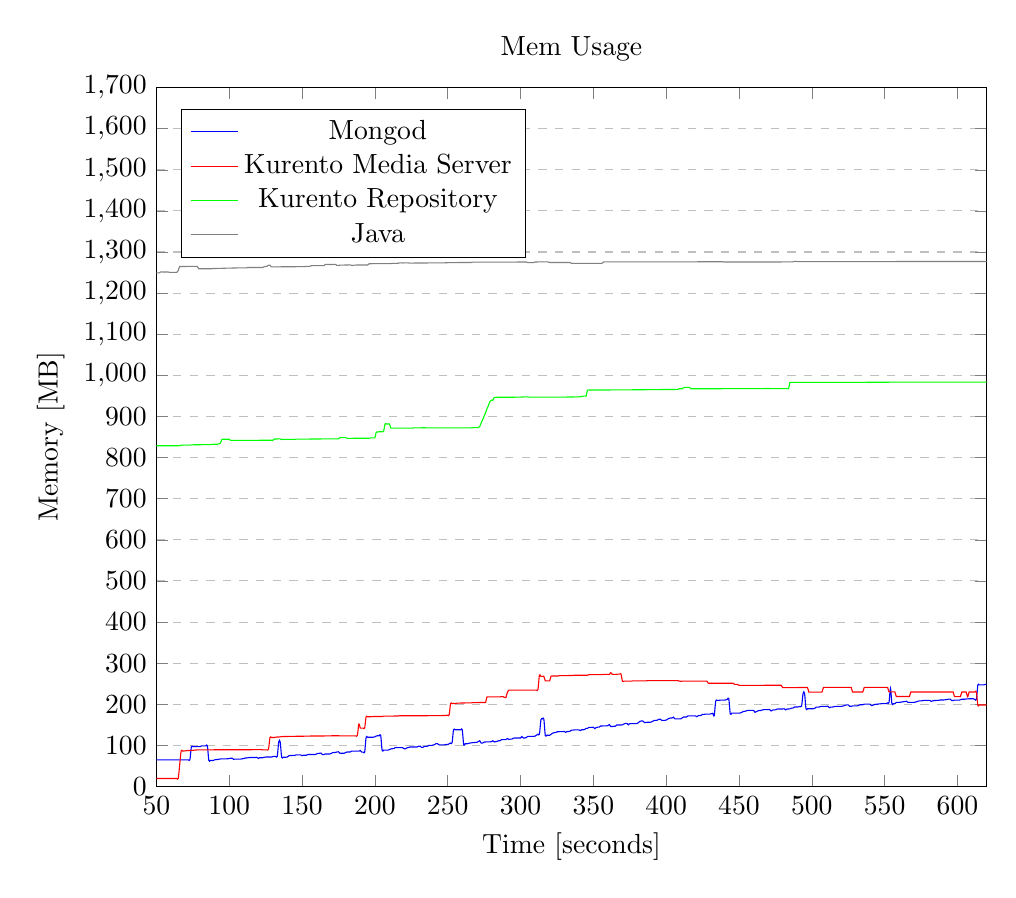
\begin{tikzpicture}
	\begin{axis}[
	    width=\textwidth,
	    title={Mem Usage},
	    xlabel={Time [seconds]},
	    ylabel={Memory [MB]},
	    xmin=50, xmax=620,
	    ymin=0, ymax=1700,
	    xtick={0,50,...,10000},
	    ytick={0,100,...,10000},
	    legend pos=north west,
	    ymajorgrids=true,
	    grid style=dashed,
	] 
		\addplot[smooth,color=blue]
		coordinates {
(0,43.491328)(1,43.491328)(2,43.491328)(3,43.491328)(4,44.634112)(5,44.634112)(6,44.634112)(7,44.634112)(8,44.634112)(9,44.634112)(10,44.634112)(11,44.634112)(12,44.634112)(13,44.634112)(14,81.031168)(15,81.031168)(16,81.031168)(17,81.031168)(18,81.031168)(19,81.031168)(20,81.031168)(21,81.031168)(22,81.031168)(23,81.031168)(24,81.031168)(25,81.031168)(26,81.031168)(27,81.031168)(28,81.031168)(29,81.031168)(30,81.031168)(31,81.031168)(32,81.031168)(33,81.031168)(34,81.031168)(35,81.031168)(36,81.031168)(37,81.031168)(38,81.031168)(39,81.031168)(40,81.031168)(41,81.031168)(42,81.031168)(43,81.031168)(44,97.005568)(45,64.970752)(46,64.970752)(47,64.970752)(48,64.970752)(49,64.970752)(50,64.970752)(51,64.970752)(52,64.970752)(53,64.970752)(54,64.970752)(55,64.970752)(56,64.970752)(57,64.970752)(58,64.970752)(59,64.970752)(60,64.970752)(61,64.970752)(62,64.970752)(63,64.970752)(64,64.970752)(65,64.970752)(66,64.970752)(67,64.970752)(68,64.970752)(69,64.970752)(70,64.970752)(71,64.970752)(72,64.970752)(73,64.970752)(74,96.29696)(75,96.886784)(76,96.886784)(77,96.886784)(78,96.886784)(79,96.886784)(80,96.886784)(81,98.799616)(82,98.799616)(83,98.799616)(84,98.799616)(85,99.332096)(86,63.340544)(87,63.340544)(88,63.340544)(89,63.340544)(90,64.753664)(91,65.683456)(92,65.683456)(93,66.400256)(94,67.059712)(95,67.059712)(96,67.059712)(97,67.059712)(98,67.059712)(99,67.571712)(100,68.104192)(101,68.87424)(102,68.87424)(103,66.146304)(104,66.781184)(105,66.781184)(106,66.781184)(107,66.781184)(108,66.781184)(109,67.477504)(110,68.009984)(111,69.40672)(112,69.40672)(113,69.992448)(114,70.496256)(115,70.496256)(116,70.496256)(117,70.496256)(118,70.496256)(119,71.00416)(120,68.427776)(121,70.057984)(122,70.057984)(123,70.057984)(124,71.139328)(125,71.671808)(126,71.671808)(127,71.671808)(128,71.671808)(129,71.671808)(130,72.716288)(131,73.4208)(132,73.4208)(133,73.4208)(134,108.457984)(135,108.457984)(136,71.254016)(137,71.254016)(138,71.254016)(139,71.254016)(140,71.888896)(141,74.801152)(142,75.333632)(143,75.333632)(144,75.83744)(145,75.83744)(146,76.898304)(147,76.898304)(148,76.898304)(149,76.898304)(150,75.042816)(151,76.120064)(152,76.120064)(153,76.120064)(154,77.807616)(155,77.807616)(156,77.807616)(157,77.807616)(158,77.807616)(159,77.807616)(160,79.384576)(161,80.777216)(162,80.777216)(163,81.36704)(164,77.6192)(165,77.6192)(166,79.204352)(167,79.204352)(168,79.204352)(169,79.204352)(170,80.375808)(171,82.358272)(172,82.681856)(173,82.948096)(174,84.04992)(175,84.578304)(176,80.994304)(177,80.994304)(178,80.994304)(179,80.994304)(180,82.952192)(181,83.972096)(182,83.972096)(183,83.972096)(184,85.97504)(185,85.97504)(186,85.97504)(187,85.97504)(188,85.97504)(189,85.97504)(190,87.523328)(191,83.70176)(192,83.70176)(193,83.70176)(194,119.947264)(195,119.947264)(196,119.947264)(197,119.947264)(198,119.947264)(199,119.947264)(200,120.963072)(201,122.90048)(202,123.4944)(203,123.4944)(204,124.526592)(205,87.711744)(206,88.563712)(207,88.563712)(208,88.563712)(209,88.563712)(210,89.673728)(211,91.512832)(212,92.020736)(213,92.020736)(214,94.588928)(215,94.588928)(216,94.588928)(217,94.588928)(218,94.588928)(219,94.588928)(220,91.97568)(221,91.97568)(222,94.08512)(223,94.674944)(224,96.239616)(225,96.239616)(226,96.239616)(227,96.239616)(228,96.239616)(229,96.239616)(230,97.816576)(231,98.349056)(232,95.297536)(233,95.297536)(234,97.779712)(235,97.779712)(236,97.779712)(237,100.110336)(238,100.110336)(239,100.110336)(240,100.614144)(241,102.182912)(242,104.189952)(243,104.189952)(244,101.453824)(245,101.453824)(246,101.453824)(247,101.453824)(248,101.453824)(249,102.068224)(250,102.068224)(251,103.911424)(252,105.684992)(253,106.274816)(254,137.719808)(255,137.986048)(256,137.986048)(257,137.986048)(258,137.986048)(259,137.986048)(260,137.986048)(261,101.167104)(262,104.030208)(263,104.030208)(264,104.292352)(265,105.598976)(266,106.12736)(267,106.63936)(268,106.63936)(269,107.409408)(270,107.409408)(271,109.264896)(272,111.202304)(273,105.61536)(274,105.61536)(275,108.089344)(276,108.351488)(277,108.621824)(278,108.621824)(279,108.621824)(280,109.105152)(281,111.230976)(282,108.429312)(283,109.084672)(284,109.842432)(285,111.435776)(286,111.435776)(287,114.151424)(288,114.151424)(289,114.151424)(290,114.151424)(291,116.789248)(292,114.475008)(293,115.175424)(294,115.175424)(295,117.399552)(296,117.932032)(297,117.932032)(298,117.932032)(299,117.932032)(300,117.932032)(301,121.626624)(302,118.04672)(303,118.04672)(304,119.177216)(305,122.077184)(306,122.077184)(307,122.077184)(308,122.077184)(309,122.077184)(310,122.556416)(311,124.796928)(312,127.193088)(313,127.193088)(314,162.254848)(315,164.37248)(316,164.37248)(317,124.637184)(318,124.637184)(319,124.637184)(320,124.637184)(321,127.041536)(322,129.826816)(323,130.912256)(324,130.912256)(325,133.091328)(326,133.091328)(327,133.603328)(328,133.603328)(329,133.603328)(330,134.098944)(331,131.719168)(332,133.742592)(333,133.742592)(334,134.488064)(335,137.109504)(336,137.109504)(337,137.773056)(338,137.773056)(339,137.773056)(340,137.773056)(341,135.954432)(342,138.039296)(343,138.039296)(344,138.616832)(345,141.533184)(346,141.533184)(347,143.745024)(348,143.745024)(349,143.745024)(350,144.252928)(351,140.648448)(352,143.52384)(353,144.310272)(354,144.310272)(355,147.08736)(356,147.08736)(357,147.57888)(358,147.57888)(359,147.57888)(360,148.099072)(361,150.740992)(362,145.895424)(363,145.895424)(364,146.51392)(365,146.51392)(366,149.495808)(367,149.495808)(368,149.495808)(369,149.495808)(370,150.05696)(371,152.031232)(372,153.595904)(373,153.595904)(374,150.147072)(375,152.90368)(376,152.90368)(377,152.90368)(378,152.90368)(379,152.90368)(380,153.165824)(381,155.541504)(382,158.564352)(383,159.41632)(384,159.41632)(385,155.652096)(386,155.652096)(387,156.30336)(388,156.30336)(389,156.30336)(390,157.06112)(391,159.17056)(392,160.899072)(393,160.899072)(394,161.452032)(395,163.549184)(396,163.549184)(397,160.903168)(398,160.903168)(399,160.903168)(400,161.529856)(401,163.90144)(402,165.80608)(403,166.588416)(404,166.588416)(405,168.706048)(406,164.41344)(407,164.41344)(408,164.41344)(409,164.41344)(410,164.41344)(411,166.912)(412,169.10336)(413,169.10336)(414,169.10336)(415,171.880448)(416,171.880448)(417,171.880448)(418,171.880448)(419,171.880448)(420,171.880448)(421,169.869312)(422,172.105728)(423,172.597248)(424,173.129728)(425,175.509504)(426,175.509504)(427,176.021504)(428,176.021504)(429,176.021504)(430,176.021504)(431,177.045504)(432,178.098176)(433,172.392448)(434,207.622144)(435,209.46944)(436,209.46944)(437,209.98144)(438,209.98144)(439,209.98144)(440,209.98144)(441,210.7392)(442,212.058112)(443,213.815296)(444,176.49664)(445,178.470912)(446,178.470912)(447,178.470912)(448,178.470912)(449,178.470912)(450,178.470912)(451,178.950144)(452,180.527104)(453,182.382592)(454,182.94784)(455,183.88992)(456,185.131008)(457,185.131008)(458,185.131008)(459,185.131008)(460,185.131008)(461,180.338688)(462,182.308864)(463,184.041472)(464,184.79104)(465,184.79104)(466,186.355712)(467,186.888192)(468,186.888192)(469,186.888192)(470,186.888192)(471,187.588608)(472,183.656448)(473,185.69216)(474,186.53184)(475,186.53184)(476,188.096512)(477,188.628992)(478,188.628992)(479,188.628992)(480,188.628992)(481,189.128704)(482,186.486784)(483,188.522496)(484,188.522496)(485,189.079552)(486,190.660608)(487,190.660608)(488,193.3312)(489,193.3312)(490,193.3312)(491,193.8432)(492,194.90816)(493,196.001792)(494,226.148352)(495,227.049472)(496,189.231104)(497,189.231104)(498,189.231104)(499,189.231104)(500,189.231104)(501,189.231104)(502,190.27968)(503,193.097728)(504,193.097728)(505,193.097728)(506,194.850816)(507,194.850816)(508,194.850816)(509,194.850816)(510,194.850816)(511,195.428352)(512,191.680512)(513,193.253376)(514,193.253376)(515,193.806336)(516,194.850816)(517,194.850816)(518,194.850816)(519,194.850816)(520,194.850816)(521,195.362816)(522,196.427776)(523,197.926912)(524,198.520832)(525,198.520832)(526,195.141632)(527,195.141632)(528,196.001792)(529,196.001792)(530,196.001792)(531,196.001792)(532,197.046272)(533,198.746112)(534,198.746112)(535,198.746112)(536,200.343552)(537,200.343552)(538,200.343552)(539,200.343552)(540,200.343552)(541,196.75136)(542,197.787648)(543,199.442432)(544,200.00768)(545,200.00768)(546,201.060352)(547,201.060352)(548,201.572352)(549,201.572352)(550,201.572352)(551,201.572352)(552,203.472896)(553,204.443648)(554,238.915584)(555,200.998912)(556,201.641984)(557,201.641984)(558,204.644352)(559,204.644352)(560,204.644352)(561,205.152256)(562,205.684736)(563,206.491648)(564,206.491648)(565,207.384576)(566,204.599296)(567,204.599296)(568,204.599296)(569,204.599296)(570,204.599296)(571,205.262848)(572,206.123008)(573,207.552512)(574,208.379904)(575,208.379904)(576,208.900096)(577,209.412096)(578,209.412096)(579,209.412096)(580,209.412096)(581,209.412096)(582,207.024128)(583,208.326656)(584,209.117184)(585,209.117184)(586,209.57184)(587,209.57184)(588,210.399232)(589,210.399232)(590,210.399232)(591,210.661376)(592,211.18976)(593,211.787776)(594,212.475904)(595,212.475904)(596,209.178624)(597,209.178624)(598,210.071552)(599,210.071552)(600,210.071552)(601,210.071552)(602,210.915328)(603,212.320256)(604,212.320256)(605,212.320256)(606,212.905984)(607,213.168128)(608,213.430272)(609,213.430272)(610,213.430272)(611,213.430272)(612,211.152896)(613,212.713472)(614,247.185408)(615,247.185408)(616,247.185408)(617,247.185408)(618,247.185408)(619,248.430592)(620,248.430592)(621,248.430592)(622,248.430592)(623,248.430592)(624,248.430592)(625,248.430592)(626,248.430592)(627,248.430592)(628,248.430592)(629,248.430592)(630,248.430592)(631,248.430592)(632,248.430592)(633,248.430592)(634,248.430592)(635,248.430592)(636,248.430592)(637,248.430592)(638,248.430592)(639,248.430592)(640,248.430592)(641,248.430592)(642,248.430592)(643,248.430592)(644,248.430592)(645,248.430592)(646,248.430592)(647,248.430592)(648,248.430592)(649,248.430592)(650,248.430592)(651,248.430592)(652,248.430592)(653,248.430592)(654,248.430592)(655,248.430592)
		};	
		\addlegendentry{Mongod}

		\addplot[smooth,color=red]
		coordinates {
(0,12.500992)(1,19.623936)(2,19.623936)(3,19.623936)(4,19.623936)(5,19.623936)(6,19.623936)(7,19.623936)(8,19.623936)(9,19.623936)(10,19.623936)(11,19.623936)(12,19.623936)(13,19.623936)(14,19.623936)(15,19.623936)(16,19.623936)(17,19.623936)(18,19.623936)(19,19.623936)(20,19.623936)(21,19.623936)(22,19.623936)(23,19.623936)(24,19.623936)(25,19.623936)(26,19.623936)(27,19.623936)(28,19.623936)(29,19.623936)(30,19.623936)(31,19.623936)(32,19.623936)(33,19.623936)(34,19.623936)(35,19.623936)(36,19.623936)(37,19.623936)(38,19.623936)(39,19.623936)(40,19.623936)(41,19.623936)(42,19.623936)(43,19.623936)(44,19.623936)(45,19.623936)(46,19.623936)(47,19.623936)(48,19.623936)(49,19.623936)(50,19.623936)(51,19.623936)(52,19.623936)(53,19.623936)(54,19.623936)(55,19.623936)(56,19.623936)(57,19.623936)(58,19.623936)(59,19.623936)(60,19.623936)(61,19.623936)(62,19.623936)(63,19.623936)(64,19.623936)(65,19.623936)(66,53.252096)(67,86.454272)(68,86.454272)(69,86.454272)(70,86.720512)(71,87.53152)(72,87.53152)(73,87.53152)(74,87.801856)(75,87.801856)(76,88.485888)(77,88.756224)(78,89.02656)(79,89.02656)(80,89.02656)(81,89.02656)(82,89.02656)(83,89.02656)(84,89.02656)(85,89.02656)(86,89.186304)(87,89.186304)(88,89.186304)(89,89.186304)(90,89.45664)(91,89.45664)(92,89.45664)(93,89.45664)(94,89.45664)(95,89.45664)(96,89.534464)(97,89.534464)(98,89.534464)(99,89.534464)(100,89.534464)(101,89.534464)(102,89.534464)(103,89.534464)(104,89.534464)(105,89.534464)(106,89.47712)(107,89.47712)(108,89.47712)(109,89.47712)(110,89.47712)(111,89.47712)(112,89.47712)(113,89.47712)(114,89.47712)(115,89.47712)(116,89.604096)(117,89.604096)(118,89.604096)(119,89.604096)(120,89.604096)(121,89.604096)(122,89.604096)(123,89.165824)(124,89.165824)(125,89.165824)(126,89.174016)(127,91.365376)(128,119.250944)(129,119.250944)(130,119.0912)(131,119.0912)(132,120.168448)(133,120.438784)(134,120.438784)(135,120.70912)(136,121.30304)(137,121.561088)(138,121.561088)(139,121.561088)(140,121.561088)(141,121.831424)(142,121.831424)(143,121.831424)(144,121.831424)(145,121.831424)(146,122.2656)(147,122.277888)(148,122.277888)(149,122.277888)(150,122.277888)(151,122.277888)(152,122.548224)(153,122.548224)(154,122.548224)(155,122.548224)(156,122.904576)(157,122.896384)(158,122.896384)(159,122.896384)(160,122.896384)(161,122.896384)(162,122.896384)(163,122.896384)(164,122.896384)(165,122.896384)(166,123.072512)(167,123.031552)(168,123.031552)(169,123.297792)(170,123.297792)(171,123.568128)(172,123.568128)(173,123.568128)(174,123.568128)(175,123.568128)(176,123.076608)(177,123.035648)(178,123.035648)(179,123.035648)(180,123.035648)(181,123.035648)(182,123.035648)(183,123.035648)(184,123.035648)(185,123.035648)(186,123.052032)(187,123.027456)(188,124.219392)(189,152.10496)(190,142.11072)(191,142.11072)(192,142.11072)(193,142.37696)(194,169.680896)(195,169.680896)(196,169.709568)(197,169.693184)(198,169.96352)(199,170.233856)(200,170.233856)(201,170.233856)(202,170.233856)(203,170.233856)(204,170.233856)(205,170.233856)(206,171.339776)(207,171.323392)(208,171.323392)(209,171.323392)(210,171.323392)(211,171.323392)(212,171.323392)(213,171.323392)(214,171.593728)(215,171.593728)(216,171.593728)(217,172.228608)(218,172.228608)(219,172.228608)(220,172.228608)(221,172.228608)(222,172.228608)(223,172.228608)(224,172.228608)(225,172.228608)(226,172.228608)(227,172.21632)(228,172.21632)(229,172.21632)(230,172.21632)(231,172.21632)(232,172.21632)(233,172.21632)(234,172.21632)(235,172.21632)(236,172.21632)(237,172.310528)(238,172.310528)(239,172.310528)(240,172.310528)(241,172.310528)(242,172.310528)(243,172.310528)(244,172.580864)(245,172.580864)(246,172.580864)(247,172.814336)(248,172.814336)(249,172.814336)(250,173.617152)(251,173.99808)(252,201.846784)(253,201.846784)(254,201.846784)(255,201.846784)(256,202.38336)(257,202.79296)(258,202.79296)(259,203.063296)(260,203.063296)(261,203.063296)(262,203.333632)(263,203.333632)(264,203.333632)(265,203.333632)(266,203.333632)(267,204.029952)(268,204.029952)(269,204.029952)(270,204.029952)(271,204.300288)(272,204.300288)(273,204.300288)(274,204.300288)(275,204.300288)(276,204.570624)(277,218.046464)(278,218.046464)(279,218.046464)(280,218.046464)(281,218.046464)(282,218.046464)(283,218.046464)(284,218.046464)(285,218.046464)(286,218.046464)(287,218.722304)(288,218.722304)(289,216.608768)(290,216.510464)(291,229.515264)(292,234.422272)(293,234.422272)(294,234.422272)(295,234.422272)(296,234.422272)(297,234.356736)(298,234.356736)(299,234.356736)(300,234.356736)(301,234.356736)(302,234.356736)(303,234.356736)(304,234.356736)(305,234.35264)(306,234.35264)(307,234.561536)(308,234.561536)(309,234.561536)(310,234.561536)(311,234.561536)(312,236.35968)(313,271.568896)(314,267.96032)(315,267.96032)(316,268.22656)(317,257.056768)(318,257.011712)(319,257.011712)(320,257.011712)(321,268.632064)(322,268.9024)(323,268.9024)(324,268.9024)(325,268.9024)(326,268.9024)(327,269.80352)(328,269.7216)(329,269.7216)(330,269.7216)(331,269.7216)(332,269.7216)(333,269.991936)(334,269.991936)(335,269.991936)(336,270.262272)(337,270.70464)(338,270.721024)(339,270.721024)(340,270.721024)(341,270.721024)(342,270.721024)(343,270.721024)(344,270.721024)(345,270.721024)(346,270.721024)(347,271.847424)(348,272.154624)(349,272.154624)(350,272.154624)(351,272.154624)(352,272.154624)(353,272.154624)(354,272.154624)(355,272.154624)(356,272.154624)(357,272.756736)(358,272.637952)(359,272.637952)(360,272.637952)(361,272.637952)(362,276.987904)(363,272.830464)(364,272.830464)(365,272.920576)(366,272.920576)(367,273.403904)(368,273.371136)(369,273.371136)(370,256.167936)(371,256.167936)(372,256.167936)(373,256.167936)(374,256.167936)(375,256.167936)(376,256.167936)(377,256.913408)(378,256.782336)(379,256.782336)(380,256.782336)(381,256.782336)(382,256.782336)(383,256.782336)(384,256.782336)(385,256.782336)(386,256.782336)(387,257.462272)(388,257.396736)(389,257.396736)(390,257.396736)(391,257.396736)(392,257.396736)(393,257.396736)(394,257.396736)(395,257.396736)(396,257.396736)(397,257.687552)(398,257.585152)(399,257.585152)(400,257.585152)(401,257.585152)(402,257.585152)(403,257.585152)(404,257.585152)(405,257.585152)(406,257.585152)(407,257.61792)(408,257.548288)(409,256.503808)(410,255.746048)(411,256.28672)(412,256.28672)(413,256.28672)(414,256.28672)(415,256.28672)(416,256.28672)(417,256.32768)(418,256.237568)(419,256.237568)(420,256.237568)(421,256.237568)(422,256.237568)(423,256.237568)(424,256.237568)(425,256.237568)(426,256.237568)(427,256.237568)(428,256.167936)(429,250.904576)(430,251.199488)(431,251.199488)(432,251.199488)(433,251.199488)(434,251.199488)(435,251.199488)(436,251.199488)(437,251.199488)(438,251.203584)(439,251.203584)(440,251.203584)(441,251.203584)(442,251.203584)(443,251.203584)(444,251.203584)(445,251.203584)(446,251.203584)(447,248.233984)(448,248.373248)(449,248.373248)(450,246.00576)(451,246.00576)(452,246.00576)(453,246.00576)(454,246.00576)(455,246.00576)(456,246.00576)(457,246.00576)(458,246.042624)(459,246.042624)(460,246.042624)(461,246.042624)(462,246.042624)(463,246.042624)(464,246.042624)(465,246.042624)(466,246.042624)(467,246.042624)(468,246.247424)(469,246.247424)(470,246.247424)(471,246.247424)(472,246.247424)(473,246.247424)(474,246.247424)(475,246.247424)(476,246.247424)(477,246.247424)(478,246.239232)(479,246.239232)(480,240.410624)(481,240.410624)(482,240.410624)(483,240.410624)(484,240.410624)(485,240.410624)(486,240.410624)(487,240.410624)(488,240.386048)(489,240.386048)(490,240.386048)(491,240.9472)(492,240.9472)(493,240.9472)(494,240.9472)(495,240.9472)(496,240.9472)(497,240.9472)(498,229.6832)(499,229.6832)(500,229.6832)(501,229.6832)(502,229.6832)(503,229.6832)(504,229.6832)(505,229.6832)(506,229.679104)(507,229.679104)(508,241.033216)(509,241.033216)(510,241.033216)(511,241.033216)(512,241.033216)(513,241.033216)(514,241.033216)(515,241.033216)(516,241.033216)(517,241.033216)(518,241.0496)(519,241.016832)(520,241.016832)(521,241.016832)(522,241.016832)(523,241.016832)(524,241.016832)(525,241.016832)(526,241.016832)(527,241.016832)(528,229.789696)(529,229.76512)(530,229.76512)(531,229.76512)(532,229.76512)(533,229.76512)(534,229.76512)(535,229.76512)(536,241.115136)(537,241.115136)(538,241.13152)(539,241.102848)(540,241.102848)(541,241.102848)(542,241.102848)(543,241.102848)(544,241.102848)(545,241.102848)(546,241.102848)(547,241.102848)(548,241.258496)(549,241.21344)(550,241.21344)(551,241.21344)(552,241.21344)(553,230.027264)(554,230.027264)(555,230.027264)(556,230.027264)(557,230.027264)(558,218.841088)(559,218.84928)(560,218.84928)(561,218.84928)(562,218.84928)(563,218.84928)(564,218.84928)(565,218.84928)(566,218.84928)(567,218.84928)(568,229.863424)(569,229.871616)(570,229.871616)(571,229.871616)(572,229.871616)(573,229.871616)(574,229.871616)(575,229.871616)(576,229.871616)(577,229.871616)(578,229.875712)(579,229.871616)(580,229.871616)(581,229.871616)(582,229.871616)(583,229.871616)(584,229.871616)(585,229.871616)(586,229.871616)(587,229.871616)(588,229.871616)(589,229.871616)(590,229.871616)(591,229.871616)(592,229.871616)(593,229.871616)(594,229.871616)(595,229.871616)(596,229.871616)(597,229.871616)(598,218.5216)(599,218.529792)(600,218.529792)(601,218.529792)(602,218.529792)(603,229.879808)(604,229.879808)(605,229.879808)(606,229.879808)(607,218.529792)(608,229.879808)(609,229.879808)(610,229.879808)(611,229.879808)(612,229.879808)(613,229.879808)(614,197.087232)(615,198.254592)(616,198.254592)(617,198.254592)(618,198.254592)(619,198.254592)(620,198.254592)(621,198.254592)(622,198.254592)(623,198.254592)(624,198.254592)(625,198.254592)(626,198.254592)(627,198.254592)(628,198.254592)(629,198.176768)(630,198.176768)(631,198.176768)(632,198.176768)(633,198.176768)(634,198.176768)(635,198.176768)(636,198.176768)(637,198.176768)(638,198.176768)(639,198.176768)(640,198.176768)(641,198.176768)(642,198.176768)(643,198.176768)(644,198.176768)(645,198.176768)(646,198.176768)(647,198.176768)(648,198.176768)(649,198.176768)(650,198.176768)(651,198.176768)(652,198.176768)(653,198.176768)(654,198.176768)(655,198.176768)
		};
		\addlegendentry{Kurento Media Server}

		\addplot[smooth,color=green]
		coordinates {
(0,1.59744)(1,118.984704)(2,308.604928)(3,598.867968)(4,726.593536)(5,812.105728)(6,803.446784)(7,803.446784)(8,803.446784)(9,803.446784)(10,803.446784)(11,803.524608)(12,803.65568)(13,803.65568)(14,875.515904)(15,883.503104)(16,881.664)(17,881.664)(18,881.664)(19,881.664)(20,881.664)(21,832.868352)(22,832.868352)(23,832.868352)(24,832.868352)(25,832.868352)(26,832.868352)(27,832.868352)(28,832.868352)(29,832.868352)(30,832.868352)(31,832.868352)(32,832.868352)(33,832.868352)(34,832.868352)(35,832.868352)(36,832.868352)(37,832.868352)(38,832.868352)(39,832.868352)(40,832.868352)(41,832.868352)(42,832.868352)(43,832.868352)(44,832.868352)(45,840.544256)(46,828.821504)(47,828.821504)(48,828.821504)(49,828.821504)(50,828.821504)(51,828.821504)(52,828.821504)(53,828.821504)(54,828.821504)(55,828.821504)(56,828.821504)(57,828.821504)(58,828.821504)(59,828.821504)(60,828.821504)(61,828.821504)(62,828.821504)(63,828.821504)(64,828.821504)(65,828.821504)(66,829.227008)(67,829.980672)(68,830.230528)(69,830.230528)(70,830.230528)(71,830.230528)(72,830.230528)(73,830.230528)(74,831.021056)(75,831.021056)(76,831.26272)(77,831.26272)(78,831.26272)(79,831.26272)(80,831.26272)(81,831.414272)(82,831.414272)(83,831.414272)(84,831.414272)(85,831.414272)(86,831.414272)(87,831.414272)(88,831.414272)(89,832.47104)(90,832.47104)(91,832.540672)(92,832.540672)(93,833.57696)(94,835.469312)(95,844.271616)(96,844.664832)(97,844.664832)(98,844.664832)(99,844.664832)(100,844.664832)(101,841.814016)(102,841.814016)(103,841.814016)(104,841.814016)(105,841.814016)(106,841.814016)(107,841.814016)(108,841.814016)(109,841.814016)(110,841.814016)(111,841.814016)(112,841.814016)(113,841.814016)(114,841.814016)(115,841.814016)(116,841.89184)(117,841.89184)(118,841.89184)(119,841.89184)(120,841.89184)(121,842.129408)(122,842.129408)(123,842.129408)(124,842.129408)(125,842.129408)(126,842.15808)(127,842.15808)(128,842.15808)(129,842.15808)(130,842.15808)(131,845.312)(132,845.312)(133,845.312)(134,845.451264)(135,845.451264)(136,843.952128)(137,844.242944)(138,844.242944)(139,844.242944)(140,844.242944)(141,844.242944)(142,844.242944)(143,844.242944)(144,844.242944)(145,844.242944)(146,845.04576)(147,845.04576)(148,845.04576)(149,845.04576)(150,845.04576)(151,845.04576)(152,845.04576)(153,845.04576)(154,845.04576)(155,845.04576)(156,845.238272)(157,845.238272)(158,845.238272)(159,845.238272)(160,845.238272)(161,845.238272)(162,845.238272)(163,845.316096)(164,845.586432)(165,845.586432)(166,845.586432)(167,845.586432)(168,845.586432)(169,845.586432)(170,845.586432)(171,845.586432)(172,845.586432)(173,845.586432)(174,845.586432)(175,845.586432)(176,848.494592)(177,848.494592)(178,848.494592)(179,848.494592)(180,848.494592)(181,846.90944)(182,846.90944)(183,846.90944)(184,846.90944)(185,846.90944)(186,847.126528)(187,847.126528)(188,847.126528)(189,847.126528)(190,847.126528)(191,847.126528)(192,847.126528)(193,847.126528)(194,847.126528)(195,847.126528)(196,847.126528)(197,847.806464)(198,847.806464)(199,847.806464)(200,847.806464)(201,862.191616)(202,862.294016)(203,862.818304)(204,862.818304)(205,862.818304)(206,863.821824)(207,881.774592)(208,881.774592)(209,881.774592)(210,881.774592)(211,871.641088)(212,871.641088)(213,871.641088)(214,871.641088)(215,871.641088)(216,871.641088)(217,871.780352)(218,871.780352)(219,871.780352)(220,871.780352)(221,871.780352)(222,871.780352)(223,871.780352)(224,871.780352)(225,871.780352)(226,871.780352)(227,872.300544)(228,872.300544)(229,872.300544)(230,872.300544)(231,872.267776)(232,872.46848)(233,872.46848)(234,872.46848)(235,872.46848)(236,872.206336)(237,872.206336)(238,872.206336)(239,872.206336)(240,872.206336)(241,872.206336)(242,872.206336)(243,872.206336)(244,872.235008)(245,872.235008)(246,872.235008)(247,872.235008)(248,872.235008)(249,872.235008)(250,872.235008)(251,872.235008)(252,872.300544)(253,872.300544)(254,872.300544)(255,872.300544)(256,872.300544)(257,872.394752)(258,872.394752)(259,872.394752)(260,872.394752)(261,872.394752)(262,872.394752)(263,872.394752)(264,872.394752)(265,872.394752)(266,872.394752)(267,872.730624)(268,872.730624)(269,872.730624)(270,872.730624)(271,872.730624)(272,875.802624)(273,884.453376)(274,892.076032)(275,900.726784)(276,909.1072)(277,918.962176)(278,926.80192)(279,936.26368)(280,939.507712)(281,939.60192)(282,946.311168)(283,946.311168)(284,946.85184)(285,946.85184)(286,946.85184)(287,946.85184)(288,946.85184)(289,946.85184)(290,946.85184)(291,946.85184)(292,946.85184)(293,946.85184)(294,946.85184)(295,946.85184)(296,946.85184)(297,947.109888)(298,947.109888)(299,947.109888)(300,947.109888)(301,947.355648)(302,947.523584)(303,947.523584)(304,947.523584)(305,947.523584)(306,946.999296)(307,947.0976)(308,947.0976)(309,947.0976)(310,947.0976)(311,947.0976)(312,947.0976)(313,947.0976)(314,947.0976)(315,947.0976)(316,947.0976)(317,947.11808)(318,947.11808)(319,947.11808)(320,947.11808)(321,947.11808)(322,947.11808)(323,947.11808)(324,947.11808)(325,947.11808)(326,947.11808)(327,947.228672)(328,947.228672)(329,947.228672)(330,947.228672)(331,947.228672)(332,947.26144)(333,947.26144)(334,947.26144)(335,947.26144)(336,947.26144)(337,947.675136)(338,947.675136)(339,947.675136)(340,947.675136)(341,948.076544)(342,948.379648)(343,949.43232)(344,949.43232)(345,949.43232)(346,964.247552)(347,964.284416)(348,964.284416)(349,964.284416)(350,964.284416)(351,964.284416)(352,964.284416)(353,964.284416)(354,964.284416)(355,964.284416)(356,964.284416)(357,964.390912)(358,964.390912)(359,964.390912)(360,964.390912)(361,964.390912)(362,964.608)(363,964.608)(364,964.608)(365,964.608)(366,964.608)(367,964.800512)(368,964.800512)(369,964.800512)(370,964.800512)(371,964.800512)(372,964.800512)(373,964.800512)(374,964.800512)(375,964.800512)(376,964.800512)(377,964.927488)(378,964.927488)(379,964.927488)(380,965.0176)(381,965.0176)(382,965.0176)(383,965.0176)(384,965.0176)(385,965.0176)(386,965.0176)(387,965.361664)(388,965.361664)(389,965.361664)(390,965.361664)(391,965.361664)(392,965.439488)(393,965.439488)(394,965.439488)(395,965.439488)(396,965.439488)(397,965.61152)(398,965.722112)(399,965.722112)(400,965.722112)(401,965.722112)(402,965.722112)(403,965.722112)(404,965.722112)(405,965.722112)(406,965.722112)(407,965.844992)(408,966.02112)(409,967.417856)(410,967.417856)(411,967.417856)(412,970.088448)(413,970.694656)(414,970.694656)(415,970.694656)(416,970.694656)(417,967.426048)(418,967.426048)(419,967.426048)(420,967.426048)(421,967.426048)(422,967.426048)(423,967.426048)(424,967.426048)(425,967.426048)(426,967.426048)(427,967.426048)(428,967.507968)(429,967.507968)(430,967.507968)(431,967.507968)(432,967.507968)(433,967.507968)(434,967.507968)(435,967.507968)(436,967.507968)(437,967.507968)(438,967.553024)(439,967.59808)(440,967.59808)(441,967.59808)(442,967.59808)(443,967.59808)(444,967.59808)(445,967.59808)(446,967.59808)(447,967.59808)(448,967.59808)(449,967.59808)(450,967.59808)(451,967.59808)(452,967.59808)(453,967.59808)(454,967.59808)(455,967.59808)(456,967.59808)(457,967.59808)(458,967.76192)(459,967.76192)(460,967.76192)(461,967.76192)(462,967.76192)(463,967.76192)(464,967.76192)(465,967.76192)(466,967.76192)(467,967.76192)(468,968.032256)(469,968.032256)(470,968.032256)(471,968.032256)(472,967.790592)(473,967.790592)(474,967.790592)(475,967.790592)(476,967.790592)(477,967.790592)(478,967.790592)(479,967.790592)(480,967.790592)(481,967.790592)(482,967.790592)(483,967.790592)(484,967.790592)(485,982.847488)(486,982.847488)(487,982.847488)(488,982.847488)(489,982.847488)(490,982.847488)(491,982.847488)(492,982.847488)(493,982.847488)(494,982.847488)(495,982.847488)(496,982.847488)(497,982.847488)(498,982.847488)(499,982.847488)(500,982.847488)(501,982.847488)(502,982.847488)(503,982.847488)(504,982.847488)(505,982.847488)(506,982.847488)(507,982.847488)(508,982.847488)(509,982.847488)(510,982.847488)(511,982.847488)(512,982.847488)(513,982.847488)(514,982.91712)(515,982.91712)(516,982.91712)(517,982.91712)(518,982.91712)(519,982.91712)(520,982.91712)(521,982.91712)(522,982.91712)(523,982.91712)(524,982.91712)(525,982.91712)(526,982.91712)(527,982.91712)(528,982.953984)(529,982.953984)(530,982.953984)(531,982.953984)(532,982.953984)(533,982.953984)(534,982.953984)(535,982.953984)(536,982.953984)(537,982.953984)(538,983.269376)(539,983.269376)(540,983.269376)(541,983.269376)(542,983.269376)(543,983.269376)(544,983.269376)(545,983.269376)(546,983.269376)(547,983.269376)(548,983.322624)(549,983.322624)(550,983.322624)(551,983.322624)(552,983.322624)(553,983.38816)(554,983.38816)(555,983.38816)(556,983.38816)(557,983.38816)(558,983.38816)(559,983.38816)(560,983.38816)(561,983.38816)(562,983.38816)(563,983.38816)(564,983.38816)(565,983.38816)(566,983.38816)(567,983.38816)(568,983.38816)(569,983.38816)(570,983.38816)(571,983.38816)(572,983.38816)(573,983.38816)(574,983.38816)(575,983.38816)(576,983.38816)(577,983.38816)(578,983.445504)(579,983.445504)(580,983.445504)(581,983.445504)(582,983.445504)(583,983.445504)(584,983.445504)(585,983.445504)(586,983.445504)(587,983.445504)(588,983.53152)(589,983.53152)(590,983.53152)(591,983.53152)(592,983.53152)(593,983.53152)(594,983.53152)(595,983.53152)(596,983.53152)(597,983.53152)(598,983.625728)(599,983.625728)(600,983.625728)(601,983.625728)(602,983.625728)(603,983.625728)(604,983.625728)(605,983.625728)(606,983.650304)(607,983.650304)(608,983.724032)(609,983.724032)(610,983.724032)(611,983.724032)(612,983.724032)(613,983.724032)(614,983.724032)(615,983.724032)(616,983.724032)(617,983.724032)(618,983.724032)(619,983.724032)(620,983.724032)(621,983.724032)(622,983.724032)(623,983.724032)(624,983.724032)(625,983.724032)(626,983.724032)(627,983.724032)(628,983.724032)(629,983.724032)(630,983.724032)(631,983.724032)(632,983.724032)(633,983.724032)(634,983.724032)(635,983.724032)(636,983.724032)(637,983.724032)(638,983.724032)(639,983.724032)(640,983.724032)(641,983.724032)(642,983.724032)(643,983.724032)(644,983.724032)(645,983.724032)(646,983.724032)(647,983.724032)(648,983.724032)(649,983.79776)(650,983.79776)(651,983.79776)(652,983.79776)(653,983.79776)(654,983.79776)(655,983.79776)
		};
		\addlegendentry{Kurento Repository}

		\addplot[smooth,color=gray]
		coordinates {
(4,89.182208)(5,172.670976)(6,314.056704)(7,414.040064)(8,484.37248)(9,551.497728)(10,571.88352)(11,578.39616)(12,592.490496)(13,601.31328)(14,628.588544)(15,667.516928)(16,674.398208)(17,678.055936)(18,675.897344)(19,723.529728)(20,755.535872)(21,768.466944)(22,776.904704)(23,791.810048)(24,801.910784)(25,820.281344)(26,920.424448)(27,939.17184)(28,948.391936)(29,1024.192512)(30,1038.516224)(31,1041.768448)(32,1052.50816)(33,1068.863488)(34,1072.676864)(35,1087.225856)(36,1093.246976)(37,1106.231296)(38,1129.82016)(39,1158.008832)(40,1195.749376)(41,1212.653568)(42,1226.989568)(43,1239.875584)(44,1240.010752)(45,1246.273536)(46,1248.755712)(47,1248.755712)(48,1248.755712)(49,1249.271808)(50,1249.275904)(51,1249.275904)(52,1249.275904)(53,1251.61472)(54,1251.524608)(55,1251.524608)(56,1251.524608)(57,1251.524608)(58,1251.524608)(59,1250.480128)(60,1250.480128)(61,1250.480128)(62,1250.480128)(63,1250.480128)(64,1250.418688)(65,1255.19872)(66,1264.754688)(67,1264.771072)(68,1264.771072)(69,1264.738304)(70,1264.738304)(71,1264.963584)(72,1264.971776)(73,1264.971776)(74,1264.971776)(75,1264.984064)(76,1265.045504)(77,1265.0496)(78,1265.0496)(79,1259.323392)(80,1259.323392)(81,1259.37664)(82,1259.37664)(83,1259.37664)(84,1259.37664)(85,1259.37664)(86,1259.409408)(87,1259.409408)(88,1259.409408)(89,1259.945984)(90,1259.945984)(91,1259.945984)(92,1260.09344)(93,1260.09344)(94,1260.09344)(95,1260.09344)(96,1260.531712)(97,1260.535808)(98,1260.76928)(99,1260.76928)(100,1260.802048)(101,1260.802048)(102,1261.047808)(103,1261.047808)(104,1261.047808)(105,1261.24032)(106,1261.551616)(107,1261.551616)(108,1261.551616)(109,1261.559808)(110,1261.563904)(111,1261.572096)(112,1261.572096)(113,1262.379008)(114,1262.379008)(115,1262.379008)(116,1262.379008)(117,1262.379008)(118,1262.292992)(119,1262.292992)(120,1262.292992)(121,1262.292992)(122,1262.292992)(123,1262.292992)(124,1264.197632)(125,1264.82432)(126,1265.164288)(127,1267.847168)(128,1267.847168)(129,1263.783936)(130,1263.783936)(131,1263.783936)(132,1263.783936)(133,1264.050176)(134,1264.001024)(135,1264.001024)(136,1264.091136)(137,1264.095232)(138,1264.095232)(139,1264.095232)(140,1264.103424)(141,1264.103424)(142,1264.103424)(143,1264.103424)(144,1264.103424)(145,1264.103424)(146,1264.324608)(147,1264.324608)(148,1264.324608)(149,1264.324608)(150,1264.365568)(151,1264.57856)(152,1264.893952)(153,1264.893952)(154,1264.9472)(155,1264.9472)(156,1266.343936)(157,1266.880512)(158,1266.880512)(159,1266.880512)(160,1266.925568)(161,1267.027968)(162,1267.027968)(163,1267.027968)(164,1266.929664)(165,1266.929664)(166,1269.731328)(167,1269.846016)(168,1269.846016)(169,1269.649408)(170,1269.755904)(171,1269.755904)(172,1269.82144)(173,1269.82144)(174,1267.396608)(175,1267.396608)(176,1268.027392)(177,1268.269056)(178,1268.269056)(179,1268.269056)(180,1268.535296)(181,1268.535296)(182,1268.559872)(183,1268.604928)(184,1267.351552)(185,1267.351552)(186,1268.277248)(187,1268.277248)(188,1268.412416)(189,1268.412416)(190,1268.412416)(191,1268.412416)(192,1268.412416)(193,1268.412416)(194,1268.412416)(195,1268.412416)(196,1271.373824)(197,1271.382016)(198,1271.668736)(199,1271.668736)(200,1271.672832)(201,1271.672832)(202,1271.672832)(203,1271.672832)(204,1271.672832)(205,1271.672832)(206,1271.713792)(207,1271.74656)(208,1271.74656)(209,1271.906304)(210,1271.906304)(211,1271.906304)(212,1272.307712)(213,1272.54528)(214,1272.54528)(215,1272.54528)(216,1272.614912)(217,1273.638912)(218,1273.638912)(219,1273.344)(220,1273.503744)(221,1273.503744)(222,1273.503744)(223,1273.503744)(224,1273.044992)(225,1273.044992)(226,1273.044992)(227,1273.171968)(228,1273.171968)(229,1273.171968)(230,1273.171968)(231,1273.176064)(232,1273.176064)(233,1273.176064)(234,1273.176064)(235,1273.389056)(236,1273.389056)(237,1273.475072)(238,1273.475072)(239,1273.475072)(240,1273.475072)(241,1273.475072)(242,1273.475072)(243,1273.475072)(244,1273.475072)(245,1273.479168)(246,1273.479168)(247,1273.58976)(248,1273.720832)(249,1273.921536)(250,1274.036224)(251,1274.052608)(252,1274.052608)(253,1274.052608)(254,1274.052608)(255,1274.052608)(256,1274.052608)(257,1274.4704)(258,1274.4704)(259,1274.4704)(260,1274.474496)(261,1274.482688)(262,1274.482688)(263,1274.482688)(264,1274.482688)(265,1274.482688)(266,1274.482688)(267,1275.2896)(268,1275.2896)(269,1275.2896)(270,1275.2896)(271,1275.318272)(272,1275.318272)(273,1275.318272)(274,1275.318272)(275,1275.318272)(276,1275.318272)(277,1275.338752)(278,1275.346944)(279,1275.346944)(280,1275.346944)(281,1275.346944)(282,1275.346944)(283,1275.346944)(284,1275.346944)(285,1275.346944)(286,1275.346944)(287,1275.469824)(288,1275.47392)(289,1275.47392)(290,1275.559936)(291,1275.559936)(292,1275.559936)(293,1275.559936)(294,1275.559936)(295,1275.559936)(296,1275.559936)(297,1275.564032)(298,1275.641856)(299,1275.641856)(300,1275.641856)(301,1275.641856)(302,1275.641856)(303,1275.686912)(304,1275.686912)(305,1274.179584)(306,1274.179584)(307,1274.179584)(308,1274.179584)(309,1274.32704)(310,1275.838464)(311,1275.764736)(312,1275.879424)(313,1275.879424)(314,1275.879424)(315,1275.879424)(316,1275.879424)(317,1275.916288)(318,1275.916288)(319,1275.916288)(320,1274.40896)(321,1274.40896)(322,1274.40896)(323,1274.40896)(324,1274.40896)(325,1274.40896)(326,1274.40896)(327,1274.433536)(328,1274.433536)(329,1274.433536)(330,1274.437632)(331,1274.437632)(332,1274.503168)(333,1274.503168)(334,1274.503168)(335,1272.34048)(336,1272.34048)(337,1272.38144)(338,1272.38144)(339,1272.38144)(340,1272.38144)(341,1272.38144)(342,1272.38144)(343,1272.38144)(344,1272.38144)(345,1272.38144)(346,1272.38144)(347,1272.410112)(348,1272.410112)(349,1272.410112)(350,1272.410112)(351,1272.410112)(352,1272.410112)(353,1272.410112)(354,1272.410112)(355,1272.410112)(356,1272.410112)(357,1275.891712)(358,1275.904)(359,1275.904)(360,1275.904)(361,1275.904)(362,1275.904)(363,1275.904)(364,1275.904)(365,1275.904)(366,1275.904)(367,1275.904)(368,1275.904)(369,1275.904)(370,1275.904)(371,1275.904)(372,1275.912192)(373,1275.912192)(374,1275.912192)(375,1275.912192)(376,1275.912192)(377,1275.990016)(378,1275.990016)(379,1275.990016)(380,1275.990016)(381,1275.990016)(382,1276.039168)(383,1276.039168)(384,1276.039168)(385,1276.04736)(386,1276.04736)(387,1276.141568)(388,1276.141568)(389,1276.141568)(390,1276.055552)(391,1276.055552)(392,1276.055552)(393,1276.055552)(394,1276.055552)(395,1276.055552)(396,1276.055552)(397,1276.063744)(398,1276.063744)(399,1276.063744)(400,1276.030976)(401,1276.030976)(402,1276.030976)(403,1276.030976)(404,1276.030976)(405,1276.030976)(406,1276.030976)(407,1276.030976)(408,1276.030976)(409,1276.030976)(410,1276.030976)(411,1276.030976)(412,1276.092416)(413,1276.092416)(414,1276.092416)(415,1276.092416)(416,1276.092416)(417,1276.092416)(418,1276.092416)(419,1276.092416)(420,1276.092416)(421,1276.092416)(422,1276.329984)(423,1276.329984)(424,1276.329984)(425,1276.329984)(426,1276.329984)(427,1276.329984)(428,1276.338176)(429,1276.338176)(430,1276.27264)(431,1276.27264)(432,1276.27264)(433,1276.27264)(434,1276.27264)(435,1276.27264)(436,1276.27264)(437,1276.27264)(438,1276.27264)(439,1276.27264)(440,1275.682816)(441,1275.682816)(442,1275.748352)(443,1275.748352)(444,1275.748352)(445,1275.748352)(446,1275.748352)(447,1275.748352)(448,1275.748352)(449,1275.748352)(450,1275.748352)(451,1275.748352)(452,1275.748352)(453,1275.748352)(454,1275.78112)(455,1275.78112)(456,1275.78112)(457,1275.78112)(458,1275.78112)(459,1275.78112)(460,1275.78112)(461,1275.78112)(462,1275.78112)(463,1275.78112)(464,1275.78112)(465,1275.78112)(466,1275.78112)(467,1275.78112)(468,1275.846656)(469,1275.846656)(470,1275.846656)(471,1275.846656)(472,1275.846656)(473,1275.846656)(474,1275.846656)(475,1275.846656)(476,1275.846656)(477,1275.846656)(478,1275.846656)(479,1275.846656)(480,1275.916288)(481,1275.916288)(482,1275.916288)(483,1275.916288)(484,1275.916288)(485,1275.916288)(486,1275.916288)(487,1275.916288)(488,1277.333504)(489,1277.333504)(490,1276.612608)(491,1276.612608)(492,1276.612608)(493,1276.612608)(494,1276.612608)(495,1276.612608)(496,1276.612608)(497,1276.612608)(498,1276.612608)(499,1276.612608)(500,1276.612608)(501,1276.612608)(502,1276.612608)(503,1276.612608)(504,1276.612608)(505,1276.612608)(506,1276.612608)(507,1276.612608)(508,1276.616704)(509,1276.616704)(510,1276.616704)(511,1276.616704)(512,1276.616704)(513,1276.616704)(514,1276.616704)(515,1276.616704)(516,1276.616704)(517,1276.616704)(518,1276.616704)(519,1276.5184)(520,1276.5184)(521,1276.5184)(522,1276.5184)(523,1276.5184)(524,1276.5184)(525,1276.5184)(526,1276.5184)(527,1276.5184)(528,1276.5184)(529,1276.5184)(530,1276.5184)(531,1276.5184)(532,1276.5184)(533,1276.5184)(534,1276.5184)(535,1276.5184)(536,1276.5184)(537,1276.5184)(538,1276.76416)(539,1276.772352)(540,1276.772352)(541,1276.772352)(542,1276.772352)(543,1276.772352)(544,1276.772352)(545,1276.772352)(546,1276.772352)(547,1276.772352)(548,1276.776448)(549,1276.776448)(550,1276.776448)(551,1276.776448)(552,1276.776448)(553,1276.776448)(554,1276.776448)(555,1276.776448)(556,1276.776448)(557,1276.776448)(558,1276.899328)(559,1276.899328)(560,1276.899328)(561,1276.899328)(562,1276.899328)(563,1276.899328)(564,1276.899328)(565,1276.899328)(566,1276.899328)(567,1276.899328)(568,1276.899328)(569,1276.899328)(570,1276.899328)(571,1276.899328)(572,1276.899328)(573,1276.899328)(574,1276.899328)(575,1276.899328)(576,1276.899328)(577,1276.899328)(578,1276.903424)(579,1276.90752)(580,1276.90752)(581,1276.90752)(582,1276.90752)(583,1276.90752)(584,1276.90752)(585,1276.915712)(586,1276.915712)(587,1276.915712)(588,1276.915712)(589,1276.915712)(590,1276.915712)(591,1276.915712)(592,1276.915712)(593,1276.915712)(594,1276.915712)(595,1276.915712)(596,1276.915712)(597,1276.915712)(598,1276.915712)(599,1276.915712)(600,1276.915712)(601,1276.915712)(602,1276.915712)(603,1276.915712)(604,1276.915712)(605,1276.915712)(606,1276.915712)(607,1276.915712)(608,1276.923904)(609,1276.923904)(610,1276.923904)(611,1276.923904)(612,1276.923904)(613,1276.923904)(614,1276.923904)(615,1276.923904)(616,1276.923904)(617,1276.923904)(618,1276.923904)(619,1276.928)(620,1276.928)(621,1276.928)(622,1276.928)(623,1276.928)(624,1276.928)(625,1276.928)(626,1276.928)(627,1276.928)(628,1276.928)(629,1276.928)(630,1276.928)(631,1276.928)(632,1276.928)(633,1276.928)(634,1276.928)(635,1276.928)(636,1276.928)(637,1276.928)(638,1276.928)(639,1276.928)(640,1276.928)(641,1276.928)(642,1276.928)(643,1276.928)(644,1276.928)(645,1276.928)(646,1276.928)(647,1276.928)(648,1276.940288)(649,1276.944384)(650,1276.944384)(651,1276.944384)(652,1276.944384)(653,1276.944384)(654,1276.944384)(655,1276.944384)
		};
		\addlegendentry{Java}

	\end{axis}
\end{tikzpicture}



	\end{center}

	\begin{center}
	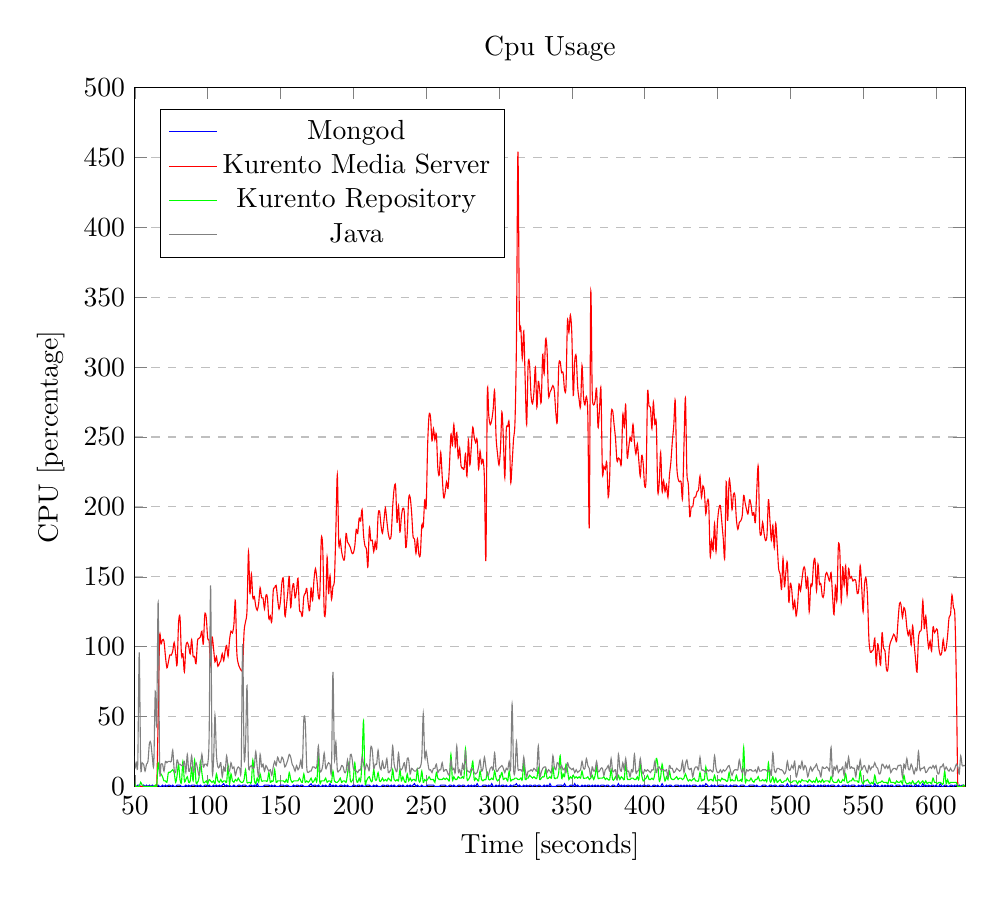
\begin{tikzpicture}
	\begin{axis}[
	    width=\textwidth,
	    title={Cpu Usage},
	    xlabel={Time [seconds]},
	    ylabel={CPU [percentage]},
	    xmin=50, xmax=620,
	    ymin=0, ymax=500,
	    xtick={0,50,...,1000},
	    ytick={0,50,...,1000},
	    legend pos=north west,
	    ymajorgrids=true,
	    grid style=dashed,
	] 
		\addplot[smooth,color=blue]
		coordinates {
(0,0.0)(1,2.0)(2,1.0)(3,0.0)(4,58.0)(5,43.0)(6,4.0)(7,29.0)(8,67.0)(9,5.0)(10,6.0)(11,88.0)(12,5.0)(13,7.0)(14,4.0)(15,0.0)(16,1.0)(17,0.0)(18,0.0)(19,1.0)(20,0.0)(21,0.0)(22,1.0)(23,0.0)(24,0.0)(25,0.0)(26,1.0)(27,0.0)(28,0.0)(29,1.0)(30,0.0)(31,1.0)(32,0.0)(33,0.0)(34,1.0)(35,0.0)(36,0.0)(37,0.0)(38,1.0)(39,0.0)(40,0.0)(41,0.0)(42,1.0)(43,0.0)(44,3.0)(45,4.0)(46,1.0)(47,1.0)(48,0.0)(49,1.0)(50,0.0)(51,0.0)(52,1.0)(53,1.0)(54,0.0)(55,0.0)(56,1.0)(57,0.0)(58,1.0)(59,0.0)(60,1.0)(61,0.0)(62,1.0)(63,0.0)(64,0.0)(65,1.0)(66,1.0)(67,0.0)(68,0.0)(69,1.0)(70,0.0)(71,1.0)(72,0.0)(73,1.0)(74,1.0)(75,0.0)(76,1.0)(77,0.0)(78,0.0)(79,1.0)(80,1.0)(81,1.0)(82,0.0)(83,0.0)(84,0.0)(85,1.0)(86,0.0)(87,1.0)(88,0.0)(89,1.0)(90,1.0)(91,1.0)(92,0.0)(93,1.0)(94,0.0)(95,1.0)(96,0.0)(97,0.0)(98,1.0)(99,1.0)(100,0.0)(101,1.0)(102,0.0)(103,0.0)(104,1.0)(105,0.0)(106,1.0)(107,0.0)(108,1.0)(109,0.0)(110,1.0)(111,2.0)(112,0.0)(113,1.0)(114,0.0)(115,1.0)(116,0.0)(117,0.0)(118,1.0)(119,0.0)(120,0.0)(121,1.0)(122,1.0)(123,0.0)(124,1.0)(125,1.0)(126,1.0)(127,0.0)(128,0.0)(129,1.0)(130,1.0)(131,0.0)(132,1.0)(133,0.0)(134,2.0)(135,0.0)(136,0.0)(137,0.0)(138,0.0)(139,1.0)(140,1.0)(141,1.0)(142,1.0)(143,0.0)(144,1.0)(145,0.0)(146,1.0)(147,0.0)(148,0.0)(149,0.0)(150,1.0)(151,1.0)(152,1.0)(153,0.0)(154,1.0)(155,1.0)(156,0.0)(157,0.0)(158,0.0)(159,1.0)(160,0.0)(161,1.0)(162,1.0)(163,0.0)(164,1.0)(165,1.0)(166,0.0)(167,0.0)(168,0.0)(169,0.0)(170,1.0)(171,2.0)(172,0.0)(173,1.0)(174,1.0)(175,0.0)(176,1.0)(177,0.0)(178,0.0)(179,1.0)(180,0.0)(181,1.0)(182,0.0)(183,0.0)(184,2.0)(185,0.0)(186,1.0)(187,0.0)(188,1.0)(189,0.0)(190,0.0)(191,1.0)(192,1.0)(193,0.0)(194,1.0)(195,0.0)(196,1.0)(197,0.0)(198,0.0)(199,0.0)(200,1.0)(201,1.0)(202,0.0)(203,1.0)(204,1.0)(205,0.0)(206,1.0)(207,0.0)(208,0.0)(209,1.0)(210,1.0)(211,1.0)(212,0.0)(213,0.0)(214,1.0)(215,0.0)(216,1.0)(217,0.0)(218,0.0)(219,0.0)(220,1.0)(221,1.0)(222,0.0)(223,1.0)(224,1.0)(225,0.0)(226,1.0)(227,0.0)(228,1.0)(229,0.0)(230,0.0)(231,1.0)(232,1.0)(233,0.0)(234,1.0)(235,0.0)(236,0.0)(237,1.0)(238,0.0)(239,1.0)(240,0.0)(241,1.0)(242,2.0)(243,0.0)(244,1.0)(245,0.0)(246,0.0)(247,1.0)(248,0.0)(249,0.0)(250,0.0)(251,1.0)(252,1.0)(253,1.0)(254,1.0)(255,1.0)(256,0.0)(257,0.0)(258,0.0)(259,0.0)(260,1.0)(261,1.0)(262,1.0)(263,1.0)(264,0.0)(265,0.0)(266,1.0)(267,1.0)(268,0.0)(269,1.0)(270,0.0)(271,0.0)(272,1.0)(273,1.0)(274,0.0)(275,1.0)(276,1.0)(277,0.0)(278,0.0)(279,1.0)(280,0.0)(281,1.0)(282,0.0)(283,1.0)(284,0.0)(285,2.0)(286,0.0)(287,0.0)(288,0.0)(289,1.0)(290,1.0)(291,1.0)(292,0.0)(293,1.0)(294,0.0)(295,2.0)(296,0.0)(297,0.0)(298,1.0)(299,0.0)(300,1.0)(301,0.0)(302,1.0)(303,1.0)(304,0.0)(305,1.0)(306,0.0)(307,0.0)(308,1.0)(309,0.0)(310,1.0)(311,1.0)(312,2.0)(313,0.0)(314,1.0)(315,0.0)(316,0.0)(317,1.0)(318,0.0)(319,1.0)(320,0.0)(321,1.0)(322,1.0)(323,0.0)(324,1.0)(325,1.0)(326,0.0)(327,1.0)(328,1.0)(329,0.0)(330,0.0)(331,1.0)(332,0.0)(333,1.0)(334,0.0)(335,2.0)(336,0.0)(337,0.0)(338,0.0)(339,0.0)(340,1.0)(341,1.0)(342,1.0)(343,1.0)(344,0.0)(345,2.0)(346,0.0)(347,0.0)(348,0.0)(349,1.0)(350,1.0)(351,0.0)(352,2.0)(353,0.0)(354,1.0)(355,0.0)(356,0.0)(357,1.0)(358,0.0)(359,1.0)(360,0.0)(361,1.0)(362,1.0)(363,0.0)(364,1.0)(365,0.0)(366,1.0)(367,0.0)(368,1.0)(369,0.0)(370,1.0)(371,1.0)(372,1.0)(373,0.0)(374,1.0)(375,1.0)(376,0.0)(377,0.0)(378,1.0)(379,1.0)(380,0.0)(381,0.0)(382,2.0)(383,0.0)(384,1.0)(385,0.0)(386,1.0)(387,0.0)(388,1.0)(389,1.0)(390,0.0)(391,1.0)(392,0.0)(393,1.0)(394,0.0)(395,1.0)(396,0.0)(397,1.0)(398,0.0)(399,1.0)(400,1.0)(401,0.0)(402,1.0)(403,1.0)(404,0.0)(405,0.0)(406,1.0)(407,1.0)(408,0.0)(409,1.0)(410,0.0)(411,0.0)(412,2.0)(413,0.0)(414,0.0)(415,1.0)(416,0.0)(417,1.0)(418,1.0)(419,0.0)(420,0.0)(421,1.0)(422,1.0)(423,1.0)(424,0.0)(425,1.0)(426,0.0)(427,1.0)(428,0.0)(429,1.0)(430,0.0)(431,1.0)(432,0.0)(433,1.0)(434,1.0)(435,1.0)(436,0.0)(437,0.0)(438,1.0)(439,0.0)(440,1.0)(441,0.0)(442,2.0)(443,1.0)(444,0.0)(445,0.0)(446,1.0)(447,0.0)(448,1.0)(449,0.0)(450,0.0)(451,1.0)(452,1.0)(453,1.0)(454,1.0)(455,0.0)(456,1.0)(457,0.0)(458,0.0)(459,1.0)(460,0.0)(461,1.0)(462,1.0)(463,1.0)(464,0.0)(465,0.0)(466,1.0)(467,1.0)(468,1.0)(469,0.0)(470,0.0)(471,0.0)(472,1.0)(473,1.0)(474,1.0)(475,1.0)(476,0.0)(477,1.0)(478,0.0)(479,0.0)(480,0.0)(481,1.0)(482,1.0)(483,1.0)(484,0.0)(485,0.0)(486,1.0)(487,1.0)(488,0.0)(489,1.0)(490,1.0)(491,0.0)(492,0.0)(493,1.0)(494,1.0)(495,1.0)(496,0.0)(497,0.0)(498,2.0)(499,0.0)(500,0.0)(501,1.0)(502,0.0)(503,1.0)(504,1.0)(505,0.0)(506,0.0)(507,1.0)(508,0.0)(509,0.0)(510,1.0)(511,0.0)(512,1.0)(513,1.0)(514,1.0)(515,0.0)(516,1.0)(517,0.0)(518,0.0)(519,1.0)(520,0.0)(521,1.0)(522,0.0)(523,1.0)(524,1.0)(525,0.0)(526,1.0)(527,0.0)(528,1.0)(529,1.0)(530,1.0)(531,0.0)(532,0.0)(533,1.0)(534,0.0)(535,0.0)(536,1.0)(537,1.0)(538,1.0)(539,0.0)(540,1.0)(541,0.0)(542,1.0)(543,1.0)(544,1.0)(545,0.0)(546,0.0)(547,1.0)(548,0.0)(549,1.0)(550,1.0)(551,0.0)(552,1.0)(553,1.0)(554,1.0)(555,1.0)(556,0.0)(557,0.0)(558,2.0)(559,0.0)(560,1.0)(561,0.0)(562,0.0)(563,1.0)(564,0.0)(565,1.0)(566,0.0)(567,1.0)(568,0.0)(569,1.0)(570,1.0)(571,0.0)(572,0.0)(573,1.0)(574,1.0)(575,1.0)(576,0.0)(577,0.0)(578,1.0)(579,0.0)(580,1.0)(581,0.0)(582,1.0)(583,1.0)(584,0.0)(585,0.0)(586,2.0)(587,0.0)(588,1.0)(589,0.0)(590,0.0)(591,2.0)(592,0.0)(593,1.0)(594,0.0)(595,1.0)(596,0.0)(597,1.0)(598,1.0)(599,0.0)(600,1.0)(601,0.0)(602,0.0)(603,2.0)(604,0.0)(605,0.0)(606,1.0)(607,1.0)(608,0.0)(609,0.0)(610,1.0)(611,1.0)(612,0.0)(613,1.0)(614,1.0)(615,0.0)(616,1.0)(617,0.0)(618,1.0)(619,1.0)(620,0.0)(621,0.0)(622,0.0)(623,1.0)(624,1.0)(625,0.0)(626,1.0)(627,0.0)(628,0.0)(629,1.0)(630,0.0)(631,1.0)(632,0.0)(633,0.0)(634,0.0)(635,1.0)(636,0.0)(637,1.0)(638,0.0)(639,0.0)(640,1.0)(641,0.0)(642,1.0)(643,1.0)(644,0.0)(645,0.0)(646,0.0)(647,1.0)(648,1.0)(649,0.0)(650,1.0)(651,0.0)(652,0.0)(653,1.0)(654,0.0)(655,1.0)
		};	
		\addlegendentry{Mongod}

		\addplot[smooth,color=red]
		coordinates {
(0,0.0)(1,11.0)(2,0.0)(3,0.0)(4,0.0)(5,0.0)(6,0.0)(7,0.0)(8,0.0)(9,0.0)(10,0.0)(11,0.0)(12,0.0)(13,0.0)(14,0.0)(15,0.0)(16,0.0)(17,0.0)(18,0.0)(19,0.0)(20,0.0)(21,0.0)(22,0.0)(23,0.0)(24,0.0)(25,0.0)(26,0.0)(27,0.0)(28,0.0)(29,0.0)(30,0.0)(31,0.0)(32,0.0)(33,0.0)(34,0.0)(35,0.0)(36,0.0)(37,0.0)(38,0.0)(39,0.0)(40,0.0)(41,0.0)(42,0.0)(43,0.0)(44,0.0)(45,0.0)(46,0.0)(47,0.0)(48,0.0)(49,0.0)(50,0.0)(51,0.0)(52,0.0)(53,0.0)(54,0.0)(55,0.0)(56,0.0)(57,0.0)(58,0.0)(59,0.0)(60,0.0)(61,0.0)(62,0.0)(63,0.0)(64,0.0)(65,0.0)(66,49.0)(67,107.0)(68,102.0)(69,105.0)(70,104.0)(71,93.1)(72,84.9)(73,89.0)(74,94.1)(75,94.0)(76,96.9)(77,103.0)(78,95.1)(79,86.9)(80,117.0)(81,121.0)(82,94.0)(83,95.0)(84,82.0)(85,100.0)(86,103.1)(87,100.0)(88,94.9)(89,105.1)(90,93.0)(91,93.0)(92,87.9)(93,104.0)(94,106.0)(95,107.0)(96,111.1)(97,102.0)(98,122.9)(99,121.0)(100,106.1)(101,104.0)(102,86.9)(103,107.0)(104,99.0)(105,89.1)(106,92.9)(107,86.0)(108,88.0)(109,90.0)(110,95.1)(111,90.0)(112,97.0)(113,100.9)(114,93.1)(115,104.9)(116,111.1)(117,109.9)(118,116.0)(119,133.0)(120,96.1)(121,87.9)(122,85.0)(123,83.1)(124,85.0)(125,110.9)(126,118.0)(127,126.1)(128,168.0)(129,137.9)(130,152.0)(131,135.0)(132,136.0)(133,129.0)(134,126.1)(135,130.9)(136,142.2)(137,135.0)(138,134.9)(139,127.1)(140,136.9)(141,135.0)(142,120.0)(143,122.1)(144,117.9)(145,139.9)(146,142.1)(147,143.9)(148,134.2)(149,126.9)(150,133.0)(151,146.1)(152,147.9)(153,122.1)(154,128.9)(155,139.0)(156,150.2)(157,128.0)(158,140.9)(159,145.1)(160,135.0)(161,140.1)(162,148.9)(163,127.1)(164,125.0)(165,122.0)(166,136.0)(167,138.1)(168,141.7)(169,131.1)(170,125.9)(171,142.0)(172,133.1)(173,148.0)(174,155.9)(175,148.0)(176,136.0)(177,137.8)(178,177.0)(179,170.2)(180,124.9)(181,127.0)(182,164.2)(183,138.0)(184,150.9)(185,133.9)(186,143.1)(187,147.9)(188,183.2)(189,223.0)(190,173.8)(191,176.2)(192,167.8)(193,163.0)(194,163.2)(195,181.0)(196,174.9)(197,173.2)(198,170.9)(199,167.1)(200,167.0)(201,172.0)(202,184.0)(203,181.0)(204,192.0)(205,189.9)(206,198.1)(207,180.0)(208,172.0)(209,170.0)(210,157.0)(211,185.0)(212,175.9)(213,176.2)(214,168.0)(215,175.0)(216,170.0)(217,193.9)(218,197.1)(219,186.8)(220,181.2)(221,190.0)(222,199.2)(223,189.9)(224,181.0)(225,177.0)(226,180.0)(227,200.0)(228,213.0)(229,215.0)(230,189.0)(231,201.0)(232,182.0)(233,193.1)(234,199.0)(235,196.0)(236,171.0)(237,181.0)(238,206.0)(239,207.0)(240,196.0)(241,179.0)(242,177.0)(243,166.8)(244,177.2)(245,166.0)(246,166.1)(247,186.9)(248,186.0)(249,205.0)(250,199.9)(251,244.0)(252,265.7)(253,264.1)(254,247.2)(255,256.0)(256,248.0)(257,252.2)(258,227.9)(259,223.0)(260,239.0)(261,222.0)(262,206.8)(263,210.2)(264,218.0)(265,213.2)(266,229.8)(267,252.0)(268,244.0)(269,259.0)(270,242.9)(271,253.1)(272,235.0)(273,242.0)(274,229.0)(275,228.0)(276,227.0)(277,238.0)(278,222.0)(279,248.0)(280,230.0)(281,243.0)(282,257.0)(283,250.0)(284,246.0)(285,248.0)(286,227.0)(287,240.0)(288,231.0)(289,234.0)(290,219.9)(291,162.1)(292,281.7)(293,265.2)(294,258.9)(295,262.1)(296,269.9)(297,283.1)(298,250.0)(299,238.0)(300,230.0)(301,241.0)(302,268.0)(303,249.0)(304,221.0)(305,255.0)(306,257.7)(307,259.3)(308,218.0)(309,231.2)(310,248.8)(311,261.2)(312,319.8)(313,454.1)(314,335.1)(315,327.9)(316,306.2)(317,325.8)(318,290.0)(319,259.0)(320,302.0)(321,302.0)(322,280.0)(323,273.8)(324,282.2)(325,300.0)(326,271.2)(327,289.8)(328,283.0)(329,274.9)(330,309.0)(331,295.1)(332,320.0)(333,312.0)(334,280.0)(335,282.0)(336,284.2)(337,286.8)(338,283.1)(339,267.8)(340,261.0)(341,300.0)(342,304.0)(343,296.0)(344,296.0)(345,284.0)(346,285.9)(347,333.0)(348,324.7)(349,337.3)(350,323.9)(351,279.8)(352,304.3)(353,307.9)(354,286.1)(355,277.0)(356,271.8)(357,301.2)(358,279.0)(359,273.0)(360,279.0)(361,265.0)(362,186.0)(363,353.0)(364,282.0)(365,273.0)(366,276.0)(367,285.0)(368,257.0)(369,269.7)(370,284.3)(371,225.0)(372,229.0)(373,227.0)(374,231.9)(375,207.0)(376,222.0)(377,265.0)(378,269.0)(379,259.1)(380,249.0)(381,233.0)(382,235.0)(383,233.8)(384,231.2)(385,266.0)(386,257.0)(387,273.0)(388,236.0)(389,242.0)(390,250.0)(391,247.0)(392,259.1)(393,246.0)(394,237.9)(395,245.0)(396,233.1)(397,221.9)(398,236.9)(399,231.0)(400,215.2)(401,220.9)(402,281.7)(403,272.2)(404,271.0)(405,256.0)(406,275.0)(407,259.0)(408,260.0)(409,211.7)(410,217.2)(411,239.0)(412,211.1)(413,218.9)(414,211.0)(415,216.0)(416,206.8)(417,222.2)(418,232.0)(419,246.7)(420,258.3)(421,276.0)(422,231.0)(423,220.0)(424,218.0)(425,218.0)(426,206.0)(427,243.9)(428,278.0)(429,225.0)(430,216.0)(431,193.0)(432,200.0)(433,200.0)(434,206.8)(435,207.0)(436,211.0)(437,212.2)(438,222.0)(439,206.8)(440,215.1)(441,211.1)(442,195.0)(443,204.0)(444,202.0)(445,165.0)(446,176.0)(447,169.0)(448,188.0)(449,168.0)(450,189.0)(451,198.8)(452,201.0)(453,189.1)(454,177.0)(455,164.0)(456,218.0)(457,190.1)(458,219.1)(459,212.9)(460,198.0)(461,209.0)(462,208.0)(463,191.0)(464,184.0)(465,188.9)(466,190.1)(467,193.8)(468,208.2)(469,202.9)(470,198.1)(471,195.0)(472,205.0)(473,201.8)(474,194.1)(475,196.0)(476,188.8)(477,212.3)(478,228.9)(479,185.0)(480,180.0)(481,189.0)(482,181.0)(483,176.0)(484,179.8)(485,205.2)(486,190.9)(487,176.1)(488,186.9)(489,170.9)(490,188.2)(491,173.0)(492,155.9)(493,152.0)(494,141.0)(495,163.2)(496,142.9)(497,153.9)(498,160.2)(499,131.9)(500,145.1)(501,140.9)(502,127.1)(503,133.0)(504,122.1)(505,129.8)(506,145.0)(507,140.0)(508,148.1)(509,155.8)(510,156.1)(511,141.9)(512,149.1)(513,125.0)(514,143.9)(515,144.1)(516,159.8)(517,162.0)(518,140.0)(519,159.1)(520,145.1)(521,145.0)(522,136.0)(523,136.9)(524,150.0)(525,153.1)(526,150.0)(527,147.0)(528,153.0)(529,136.8)(530,123.0)(531,143.9)(532,133.2)(533,172.0)(534,167.9)(535,131.9)(536,157.0)(537,144.0)(538,158.0)(539,137.0)(540,156.0)(541,149.0)(542,150.1)(543,147.0)(544,148.1)(545,146.9)(546,138.0)(547,140.9)(548,158.1)(549,143.1)(550,125.0)(551,144.9)(552,149.2)(553,135.9)(554,105.0)(555,96.0)(556,97.0)(557,98.0)(558,106.0)(559,87.0)(560,102.0)(561,96.0)(562,86.9)(563,109.9)(564,99.0)(565,97.1)(566,84.0)(567,84.0)(568,99.1)(569,103.8)(570,106.2)(571,108.9)(572,107.0)(573,104.0)(574,119.0)(575,131.0)(576,130.1)(577,120.9)(578,128.0)(579,125.0)(580,114.0)(581,108.1)(582,111.9)(583,101.1)(584,115.0)(585,102.9)(586,91.1)(587,81.9)(588,106.0)(589,111.1)(590,113.0)(591,132.9)(592,113.0)(593,122.1)(594,109.0)(595,98.9)(596,104.1)(597,96.9)(598,114.0)(599,110.1)(600,111.9)(601,112.0)(602,99.1)(603,94.0)(604,95.9)(605,105.1)(606,97.0)(607,99.0)(608,108.0)(609,120.9)(610,123.0)(611,137.0)(612,128.1)(613,122.0)(614,75.9)(615,0.0)(616,0.0)(617,0.0)(618,0.0)(619,0.0)(620,0.0)(621,0.0)(622,0.0)(623,0.0)(624,0.0)(625,0.0)(626,0.0)(627,0.0)(628,0.0)(629,0.0)(630,0.0)(631,0.0)(632,0.0)(633,0.0)(634,0.0)(635,0.0)(636,0.0)(637,0.0)(638,0.0)(639,0.0)(640,0.0)(641,0.0)(642,0.0)(643,0.0)(644,0.0)(645,0.0)(646,0.0)(647,0.0)(648,0.0)(649,0.0)(650,0.0)(651,0.0)(652,0.0)(653,0.0)(654,0.0)(655,0.0)
		};
		\addlegendentry{Kurento Media Server}

		\addplot[smooth,color=green]
		coordinates {
(0,0.0)(1,261.7)(2,367.0)(3,542.1)(4,448.9)(5,712.1)(6,33.0)(7,9.0)(8,12.0)(9,11.0)(10,4.0)(11,7.0)(12,5.0)(13,4.0)(14,502.5)(15,272.2)(16,136.8)(17,0.0)(18,0.0)(19,0.0)(20,0.0)(21,2.0)(22,0.0)(23,0.0)(24,0.0)(25,0.0)(26,0.0)(27,0.0)(28,0.0)(29,1.0)(30,0.0)(31,0.0)(32,0.0)(33,0.0)(34,0.0)(35,0.0)(36,1.0)(37,0.0)(38,0.0)(39,0.0)(40,1.0)(41,0.0)(42,0.0)(43,0.0)(44,0.0)(45,36.0)(46,0.0)(47,0.0)(48,0.0)(49,7.0)(50,1.0)(51,0.0)(52,0.0)(53,0.0)(54,3.0)(55,1.0)(56,0.0)(57,0.0)(58,0.0)(59,0.0)(60,0.0)(61,0.0)(62,0.0)(63,0.0)(64,1.0)(65,0.0)(66,17.0)(67,10.0)(68,9.0)(69,7.0)(70,4.0)(71,4.0)(72,3.0)(73,10.0)(74,10.0)(75,11.0)(76,12.0)(77,10.0)(78,3.0)(79,8.0)(80,16.0)(81,5.0)(82,3.0)(83,18.0)(84,4.0)(85,5.0)(86,7.0)(87,3.0)(88,4.0)(89,13.0)(90,4.0)(91,19.0)(92,3.0)(93,3.0)(94,6.0)(95,18.0)(96,10.0)(97,3.0)(98,3.0)(99,4.0)(100,2.0)(101,5.0)(102,4.0)(103,3.0)(104,4.0)(105,2.0)(106,9.0)(107,4.0)(108,3.0)(109,5.0)(110,3.0)(111,4.0)(112,4.0)(113,3.0)(114,15.0)(115,2.0)(116,9.0)(117,4.0)(118,3.0)(119,5.0)(120,4.0)(121,6.0)(122,4.0)(123,3.0)(124,3.0)(125,5.0)(126,12.0)(127,3.0)(128,3.0)(129,3.0)(130,3.0)(131,19.0)(132,5.0)(133,2.0)(134,6.0)(135,3.0)(136,9.0)(137,4.0)(138,4.0)(139,4.0)(140,4.0)(141,4.0)(142,10.0)(143,3.0)(144,4.0)(145,4.0)(146,12.0)(147,3.0)(148,4.0)(149,4.0)(150,4.0)(151,4.0)(152,4.0)(153,3.0)(154,5.0)(155,3.0)(156,10.0)(157,5.0)(158,3.0)(159,4.0)(160,4.0)(161,4.0)(162,4.0)(163,6.0)(164,4.0)(165,3.0)(166,9.0)(167,3.0)(168,4.0)(169,3.0)(170,4.0)(171,6.0)(172,3.0)(173,4.0)(174,6.0)(175,4.0)(176,22.0)(177,3.0)(178,4.0)(179,4.0)(180,4.0)(181,6.0)(182,3.0)(183,4.0)(184,4.0)(185,3.0)(186,11.0)(187,4.0)(188,3.0)(189,3.0)(190,4.0)(191,6.0)(192,3.0)(193,4.0)(194,4.0)(195,3.0)(196,9.0)(197,17.0)(198,4.0)(199,4.0)(200,6.0)(201,17.0)(202,5.0)(203,3.0)(204,6.0)(205,4.0)(206,19.0)(207,47.0)(208,4.0)(209,4.0)(210,6.0)(211,7.0)(212,4.0)(213,4.0)(214,12.0)(215,5.0)(216,5.0)(217,10.0)(218,4.0)(219,4.0)(220,6.0)(221,4.0)(222,5.0)(223,4.0)(224,6.0)(225,5.0)(226,4.0)(227,12.0)(228,5.0)(229,4.0)(230,5.0)(231,4.0)(232,12.0)(233,4.0)(234,7.0)(235,4.0)(236,3.0)(237,9.0)(238,4.0)(239,6.0)(240,4.0)(241,5.0)(242,5.0)(243,4.0)(244,12.0)(245,4.0)(246,4.0)(247,11.0)(248,3.0)(249,5.0)(250,4.0)(251,5.0)(252,7.0)(253,5.0)(254,5.0)(255,5.0)(256,3.0)(257,10.0)(258,6.0)(259,5.0)(260,5.0)(261,5.0)(262,6.0)(263,5.0)(264,6.0)(265,5.0)(266,5.0)(267,23.0)(268,5.0)(269,7.0)(270,5.0)(271,5.0)(272,7.0)(273,6.0)(274,6.0)(275,7.0)(276,7.0)(277,27.0)(278,6.0)(279,5.0)(280,7.0)(281,11.0)(282,18.0)(283,5.0)(284,6.0)(285,5.0)(286,4.0)(287,11.0)(288,5.0)(289,4.0)(290,5.0)(291,5.0)(292,10.0)(293,5.0)(294,5.0)(295,6.0)(296,5.0)(297,11.0)(298,6.0)(299,4.0)(300,5.0)(301,7.0)(302,10.0)(303,5.0)(304,6.0)(305,6.0)(306,4.0)(307,11.0)(308,4.0)(309,5.0)(310,5.0)(311,6.0)(312,6.0)(313,5.0)(314,5.0)(315,6.0)(316,5.0)(317,17.0)(318,5.0)(319,6.0)(320,6.0)(321,8.0)(322,7.0)(323,6.0)(324,7.0)(325,6.0)(326,6.0)(327,13.0)(328,5.0)(329,6.0)(330,7.0)(331,7.0)(332,12.0)(333,6.0)(334,6.0)(335,7.0)(336,6.0)(337,14.0)(338,6.0)(339,6.0)(340,6.0)(341,10.0)(342,22.0)(343,6.0)(344,9.0)(345,7.0)(346,16.0)(347,12.0)(348,5.0)(349,7.0)(350,6.0)(351,8.0)(352,6.0)(353,7.0)(354,6.0)(355,7.0)(356,6.0)(357,11.0)(358,6.0)(359,6.0)(360,6.0)(361,7.0)(362,5.0)(363,6.0)(364,8.0)(365,5.0)(366,8.0)(367,14.0)(368,6.0)(369,6.0)(370,6.0)(371,6.0)(372,7.0)(373,5.0)(374,6.0)(375,5.0)(376,5.0)(377,12.0)(378,5.0)(379,5.0)(380,7.0)(381,5.0)(382,8.0)(383,5.0)(384,7.0)(385,6.0)(386,5.0)(387,17.0)(388,6.0)(389,5.0)(390,5.0)(391,6.0)(392,6.0)(393,5.0)(394,5.0)(395,7.0)(396,5.0)(397,16.0)(398,8.0)(399,4.0)(400,5.0)(401,6.0)(402,8.0)(403,5.0)(404,5.0)(405,6.0)(406,5.0)(407,9.0)(408,20.0)(409,16.0)(410,4.0)(411,7.0)(412,16.0)(413,9.0)(414,4.0)(415,7.0)(416,5.0)(417,11.0)(418,6.0)(419,5.0)(420,5.0)(421,6.0)(422,7.0)(423,5.0)(424,6.0)(425,6.0)(426,5.0)(427,6.0)(428,9.0)(429,6.0)(430,4.0)(431,5.0)(432,4.0)(433,5.0)(434,6.0)(435,4.0)(436,4.0)(437,4.0)(438,10.0)(439,4.0)(440,5.0)(441,5.0)(442,14.0)(443,6.0)(444,4.0)(445,5.0)(446,5.0)(447,4.0)(448,8.0)(449,4.0)(450,4.0)(451,5.0)(452,4.0)(453,6.0)(454,5.0)(455,5.0)(456,4.0)(457,4.0)(458,10.0)(459,4.0)(460,5.0)(461,4.0)(462,4.0)(463,8.0)(464,4.0)(465,4.0)(466,5.0)(467,5.0)(468,28.0)(469,4.0)(470,5.0)(471,4.0)(472,4.0)(473,6.0)(474,4.0)(475,3.0)(476,5.0)(477,5.0)(478,7.0)(479,4.0)(480,4.0)(481,5.0)(482,4.0)(483,5.0)(484,4.0)(485,17.0)(486,4.0)(487,4.0)(488,7.0)(489,3.0)(490,6.0)(491,3.0)(492,4.0)(493,5.0)(494,3.0)(495,3.0)(496,4.0)(497,4.0)(498,6.0)(499,4.0)(500,3.0)(501,3.0)(502,4.0)(503,4.0)(504,4.0)(505,2.0)(506,4.0)(507,3.0)(508,5.0)(509,4.0)(510,4.0)(511,4.0)(512,3.0)(513,5.0)(514,4.0)(515,3.0)(516,4.0)(517,3.0)(518,6.0)(519,3.0)(520,4.0)(521,3.0)(522,5.0)(523,3.0)(524,4.0)(525,4.0)(526,4.0)(527,3.0)(528,7.0)(529,4.0)(530,3.0)(531,3.0)(532,3.0)(533,5.0)(534,3.0)(535,3.0)(536,5.0)(537,4.0)(538,9.0)(539,3.0)(540,3.0)(541,4.0)(542,4.0)(543,6.0)(544,4.0)(545,4.0)(546,4.0)(547,3.0)(548,11.0)(549,4.0)(550,2.0)(551,4.0)(552,4.0)(553,5.0)(554,3.0)(555,2.0)(556,3.0)(557,2.0)(558,8.0)(559,3.0)(560,2.0)(561,3.0)(562,3.0)(563,4.0)(564,3.0)(565,3.0)(566,3.0)(567,2.0)(568,6.0)(569,3.0)(570,3.0)(571,3.0)(572,2.0)(573,4.0)(574,3.0)(575,3.0)(576,4.0)(577,2.0)(578,8.0)(579,3.0)(580,2.0)(581,2.0)(582,3.0)(583,2.0)(584,4.0)(585,2.0)(586,2.0)(587,3.0)(588,4.0)(589,2.0)(590,3.0)(591,4.0)(592,2.0)(593,4.0)(594,2.0)(595,3.0)(596,3.0)(597,2.0)(598,6.0)(599,3.0)(600,3.0)(601,2.0)(602,3.0)(603,3.0)(604,2.0)(605,2.0)(606,11.0)(607,2.0)(608,5.0)(609,2.0)(610,3.0)(611,3.0)(612,3.0)(613,3.0)(614,3.0)(615,0.0)(616,0.0)(617,0.0)(618,0.0)(619,1.0)(620,0.0)(621,0.0)(622,0.0)(623,0.0)(624,0.0)(625,0.0)(626,1.0)(627,0.0)(628,0.0)(629,0.0)(630,0.0)(631,0.0)(632,0.0)(633,0.0)(634,0.0)(635,0.0)(636,0.0)(637,1.0)(638,0.0)(639,1.0)(640,0.0)(641,0.0)(642,0.0)(643,0.0)(644,1.0)(645,0.0)(646,0.0)(647,0.0)(648,0.0)(649,1.0)(650,0.0)(651,1.0)(652,0.0)(653,0.0)(654,0.0)(655,0.0)
		};
		\addlegendentry{Kurento Repository}

		\addplot[smooth,color=gray]
		coordinates {
(4,0.0)(5,172.0)(6,344.9)(7,476.1)(8,562.0)(9,306.0)(10,536.0)(11,192.0)(12,667.1)(13,385.0)(14,731.1)(15,653.8)(16,276.6)(17,409.5)(18,349.0)(19,682.0)(20,555.1)(21,322.0)(22,276.7)(23,300.6)(24,444.7)(25,695.0)(26,855.3)(27,1182.4)(28,1150.0)(29,1249.2)(30,1127.9)(31,1192.8)(32,1267.1)(33,1199.0)(34,731.7)(35,1178.3)(36,824.8)(37,618.0)(38,1142.7)(39,847.2)(40,872.9)(41,966.2)(42,513.1)(43,240.9)(44,208.0)(45,143.0)(46,124.9)(47,9.0)(48,16.0)(49,31.0)(50,14.0)(51,17.0)(52,17.0)(53,96.0)(54,15.0)(55,17.0)(56,16.0)(57,11.0)(58,16.0)(59,18.0)(60,31.0)(61,31.0)(62,21.0)(63,16.0)(64,68.1)(65,45.0)(66,131.9)(67,14.0)(68,16.0)(69,16.0)(70,11.0)(71,18.0)(72,17.0)(73,18.0)(74,18.0)(75,18.0)(76,26.0)(77,12.0)(78,10.0)(79,19.0)(80,16.0)(81,16.0)(82,15.0)(83,15.0)(84,18.0)(85,10.0)(86,23.0)(87,11.0)(88,13.0)(89,22.0)(90,11.0)(91,13.0)(92,17.0)(93,13.0)(94,8.0)(95,13.0)(96,23.0)(97,14.0)(98,16.0)(99,16.0)(100,16.0)(101,37.0)(102,143.8)(103,17.0)(104,18.0)(105,51.1)(106,23.0)(107,14.0)(108,14.0)(109,17.0)(110,7.0)(111,14.0)(112,11.0)(113,22.0)(114,13.0)(115,11.0)(116,17.0)(117,13.0)(118,14.0)(119,8.0)(120,12.0)(121,14.0)(122,13.0)(123,14.0)(124,102.0)(125,22.0)(126,30.0)(127,72.1)(128,16.0)(129,14.0)(130,15.0)(131,13.0)(132,14.0)(133,25.0)(134,14.0)(135,7.0)(136,23.0)(137,14.0)(138,16.0)(139,11.0)(140,15.0)(141,13.0)(142,11.0)(143,12.0)(144,8.0)(145,14.0)(146,18.0)(147,15.0)(148,21.0)(149,18.0)(150,17.0)(151,21.0)(152,19.0)(153,14.0)(154,16.0)(155,19.0)(156,23.0)(157,21.0)(158,16.0)(159,14.0)(160,11.0)(161,15.0)(162,12.0)(163,14.0)(164,19.0)(165,14.0)(166,48.0)(167,46.0)(168,14.0)(169,10.0)(170,11.0)(171,11.0)(172,14.0)(173,14.0)(174,13.0)(175,15.0)(176,29.0)(177,12.0)(178,11.0)(179,15.0)(180,24.0)(181,13.0)(182,15.0)(183,17.0)(184,16.0)(185,12.0)(186,82.0)(187,20.0)(188,32.0)(189,12.0)(190,11.0)(191,12.0)(192,15.0)(193,14.0)(194,10.0)(195,11.0)(196,19.0)(197,11.0)(198,23.0)(199,21.0)(200,13.0)(201,12.0)(202,11.0)(203,10.0)(204,12.0)(205,12.0)(206,21.0)(207,16.0)(208,12.0)(209,16.0)(210,14.0)(211,12.0)(212,28.0)(213,26.0)(214,13.0)(215,16.0)(216,16.0)(217,26.0)(218,15.0)(219,12.0)(220,18.0)(221,13.0)(222,14.0)(223,20.0)(224,10.0)(225,11.0)(226,13.0)(227,29.0)(228,16.0)(229,12.0)(230,11.0)(231,24.0)(232,13.0)(233,12.0)(234,14.0)(235,17.0)(236,11.0)(237,20.0)(238,19.0)(239,9.0)(240,13.0)(241,12.0)(242,11.0)(243,11.0)(244,13.0)(245,13.0)(246,14.0)(247,21.0)(248,52.0)(249,21.0)(250,25.0)(251,18.0)(252,12.0)(253,12.0)(254,10.0)(255,13.0)(256,13.0)(257,16.0)(258,10.0)(259,12.0)(260,12.0)(261,17.0)(262,11.0)(263,12.0)(264,12.0)(265,9.0)(266,9.0)(267,19.0)(268,12.0)(269,13.0)(270,10.0)(271,29.0)(272,11.0)(273,12.0)(274,8.0)(275,16.0)(276,12.0)(277,25.0)(278,12.0)(279,11.0)(280,10.0)(281,13.0)(282,12.0)(283,10.0)(284,9.0)(285,10.0)(286,14.0)(287,19.0)(288,11.0)(289,13.0)(290,21.0)(291,14.0)(292,8.0)(293,9.0)(294,13.0)(295,14.0)(296,12.0)(297,24.0)(298,12.0)(299,11.0)(300,13.0)(301,14.0)(302,15.0)(303,13.0)(304,10.0)(305,13.0)(306,12.0)(307,18.0)(308,13.0)(309,59.0)(310,13.0)(311,11.0)(312,32.0)(313,13.0)(314,12.0)(315,12.0)(316,11.0)(317,21.0)(318,12.0)(319,7.0)(320,11.0)(321,11.0)(322,12.0)(323,11.0)(324,13.0)(325,12.0)(326,12.0)(327,29.0)(328,8.0)(329,10.0)(330,13.0)(331,14.0)(332,14.0)(333,10.0)(334,12.0)(335,11.0)(336,10.0)(337,22.0)(338,14.0)(339,12.0)(340,17.0)(341,16.0)(342,13.0)(343,15.0)(344,12.0)(345,13.0)(346,10.0)(347,17.0)(348,14.0)(349,13.0)(350,12.0)(351,13.0)(352,10.0)(353,12.0)(354,10.0)(355,11.0)(356,12.0)(357,18.0)(358,13.0)(359,13.0)(360,20.0)(361,15.0)(362,13.0)(363,7.0)(364,14.0)(365,11.0)(366,12.0)(367,18.0)(368,11.0)(369,11.0)(370,13.0)(371,13.0)(372,8.0)(373,12.0)(374,13.0)(375,15.0)(376,11.0)(377,20.0)(378,11.0)(379,11.0)(380,12.0)(381,5.0)(382,23.0)(383,13.0)(384,11.0)(385,17.0)(386,12.0)(387,20.0)(388,11.0)(389,11.0)(390,7.0)(391,12.0)(392,11.0)(393,23.0)(394,10.0)(395,11.0)(396,12.0)(397,20.0)(398,12.0)(399,9.0)(400,12.0)(401,11.0)(402,12.0)(403,11.0)(404,10.0)(405,12.0)(406,12.0)(407,18.0)(408,10.0)(409,13.0)(410,14.0)(411,12.0)(412,12.0)(413,12.0)(414,11.0)(415,12.0)(416,7.0)(417,15.0)(418,13.0)(419,13.0)(420,10.0)(421,11.0)(422,13.0)(423,12.0)(424,11.0)(425,12.0)(426,18.0)(427,10.0)(428,16.0)(429,19.0)(430,13.0)(431,12.0)(432,13.0)(433,7.0)(434,12.0)(435,14.0)(436,14.0)(437,12.0)(438,21.0)(439,12.0)(440,12.0)(441,11.0)(442,10.0)(443,12.0)(444,11.0)(445,12.0)(446,11.0)(447,11.0)(448,22.0)(449,13.0)(450,10.0)(451,10.0)(452,12.0)(453,10.0)(454,12.0)(455,11.0)(456,12.0)(457,14.0)(458,15.0)(459,11.0)(460,8.0)(461,11.0)(462,12.0)(463,12.0)(464,12.0)(465,19.0)(466,13.0)(467,10.0)(468,13.0)(469,8.0)(470,12.0)(471,11.0)(472,12.0)(473,12.0)(474,11.0)(475,11.0)(476,12.0)(477,10.0)(478,14.0)(479,11.0)(480,11.0)(481,12.0)(482,12.0)(483,12.0)(484,11.0)(485,11.0)(486,12.0)(487,8.0)(488,24.0)(489,12.0)(490,10.0)(491,13.0)(492,13.0)(493,12.0)(494,12.0)(495,11.0)(496,9.0)(497,11.0)(498,18.0)(499,12.0)(500,12.0)(501,15.0)(502,13.0)(503,18.0)(504,7.0)(505,10.0)(506,15.0)(507,13.0)(508,18.0)(509,12.0)(510,15.0)(511,13.0)(512,7.0)(513,11.0)(514,14.0)(515,11.0)(516,13.0)(517,14.0)(518,16.0)(519,12.0)(520,11.0)(521,7.0)(522,14.0)(523,13.0)(524,13.0)(525,14.0)(526,13.0)(527,12.0)(528,28.0)(529,7.0)(530,14.0)(531,12.0)(532,15.0)(533,10.0)(534,12.0)(535,12.0)(536,14.0)(537,8.0)(538,17.0)(539,13.0)(540,21.0)(541,13.0)(542,14.0)(543,13.0)(544,13.0)(545,7.0)(546,15.0)(547,12.0)(548,19.0)(549,12.0)(550,14.0)(551,15.0)(552,12.0)(553,10.0)(554,15.0)(555,12.0)(556,14.0)(557,14.0)(558,17.0)(559,14.0)(560,13.0)(561,9.0)(562,10.0)(563,16.0)(564,15.0)(565,13.0)(566,15.0)(567,13.0)(568,15.0)(569,10.0)(570,12.0)(571,13.0)(572,13.0)(573,12.0)(574,15.0)(575,15.0)(576,15.0)(577,7.0)(578,16.0)(579,13.0)(580,20.0)(581,13.0)(582,12.0)(583,16.0)(584,13.0)(585,9.0)(586,13.0)(587,12.0)(588,25.0)(589,12.0)(590,13.0)(591,13.0)(592,14.0)(593,10.0)(594,11.0)(595,13.0)(596,14.0)(597,13.0)(598,15.0)(599,13.0)(600,15.0)(601,10.0)(602,9.0)(603,14.0)(604,14.0)(605,16.0)(606,12.0)(607,14.0)(608,12.0)(609,11.0)(610,13.0)(611,11.0)(612,11.0)(613,13.0)(614,16.0)(615,14.0)(616,9.0)(617,22.0)(618,15.0)(619,15.0)(620,15.0)(621,13.0)(622,12.0)(623,12.0)(624,8.0)(625,13.0)(626,13.0)(627,14.0)(628,13.0)(629,13.0)(630,13.0)(631,7.0)(632,15.0)(633,11.0)(634,13.0)(635,14.0)(636,11.0)(637,12.0)(638,14.0)(639,7.0)(640,13.0)(641,12.0)(642,13.0)(643,12.0)(644,13.0)(645,13.0)(646,6.0)(647,14.0)(648,14.0)(649,14.0)(650,14.0)(651,15.0)(652,12.0)(653,12.0)(654,11.0)(655,15.0)
		};
		\addlegendentry{Java}

	\end{axis}
\end{tikzpicture}


	\end{center}
\end{document}
